\documentclass[compress]{beamer}
\usepackage{ifthen,verbatim}

\newcommand{\isnote}{}
\xdefinecolor{lightyellow}{rgb}{1.,1.,0.25}
\xdefinecolor{darkblue}{rgb}{0.1,0.1,0.7}

%% Uncomment this to get annotations
%% \def\notes{\addtocounter{page}{-1}
%%            \renewcommand{\isnote}{*}
%% 	   \beamertemplateshadingbackground{lightyellow}{white}
%%            \begin{frame}
%%            \frametitle{Notes for the previous page (page \insertpagenumber)}
%%            \itemize}
%% \def\endnotes{\enditemize
%% 	      \end{frame}
%%               \beamertemplateshadingbackground{white}{white}
%%               \renewcommand{\isnote}{}}

%% Uncomment this to not get annotations
\def\notes{\comment}
\def\endnotes{\endcomment}

\setbeamertemplate{navigation symbols}{}
\setbeamertemplate{headline}{\mbox{ } \hfill
\begin{minipage}{5.5 cm}
\vspace{-0.75 cm} \small
\end{minipage} \hfill
\begin{minipage}{4.5 cm}
\vspace{-0.75 cm} \small
\begin{flushright}
\ifthenelse{\equal{\insertpagenumber}{1}}{}{Jim Pivarski \hspace{0.2 cm} \insertpagenumber\isnote/\pageref{numpages}}
\end{flushright}
\end{minipage}\mbox{\hspace{0.2 cm}}\includegraphics[height=1 cm]{../cmslogo} \hspace{0.1 cm} \includegraphics[height=1 cm]{../tamulogo} \hspace{0.01 cm} \vspace{-1.05 cm}}

\begin{document}
\begin{frame}
\vfill
\begin{center}
\textcolor{darkblue}{\Large Muon Alignment from CRAFT-2009 Tracks}

\vfill
\begin{columns}
\column{0.3\linewidth}
\begin{center}
\large
\textcolor{darkblue}{Jim Pivarski}
\end{center}
\end{columns}

\begin{columns}
\column{0.3\linewidth}
\begin{center}
\scriptsize
{\it Texas A\&M University}
\end{center}
\end{columns}

\vfill
 4 September, 2009

\end{center}
\end{frame}

%% \begin{notes}
%% \item This is the annotated version of my talk.
%% \item If you want the version that I am presenting, download the one
%% labeled ``slides'' on Indico (or just ignore these yellow pages).
%% \item The annotated version is provided for extra detail and a written
%% record of comments that I intend to make orally.
%% \item Yellow notes refer to the content on the {\it previous} page.
%% \item All other slides are identical for the two versions.
%% \end{notes}

\small

\begin{frame}
\frametitle{Outline}
\begin{itemize}\setlength{\itemsep}{0.5 cm}
\item Automated procedure for running MuonAlignmentFromReference
\item DT chamber results from CRAFT-2009
\item CSC alignment tracks in CRAFT-2009
\item Work plan for the next steps
\end{itemize}
\end{frame}

\begin{frame}
\frametitle{Automated procedure}
\begin{itemize}
\item Scripts in Alignment/MuonAlignmentAlgorithms/python
\begin{itemize}\setlength{\itemsep}{0.2 cm}
\item findQualityFiles.py: selects runs from the CMS Run Registry with
  a given magnetic field, and quality flags in chosen subsystems, such
  as ``tracker and DT'' or ``tracker and CSC''
\item createJobs.py: creates a set of directories with scripts for
  running each iteration of alignment from commandline arguments (like
  cmsDriver.py, standardizes interface)
\item gather\_cfg.py: collects muon residuals (about 50 jobs)
\item align\_cfg.py: runs MINUIT on the residuals to compute a new
  geometry (1 job, must wait for the gatherers to be done)
\item submit.sh: submits the jobs with the right
  interdependencies, including 2 or more iterations (created by createJobs.py)
\end{itemize}
\item Twiki page documenting their use still needs to be written
\item Allows us to start alignment with CRAFT-2009 using everything we
  developed for CRAFT-2008
\end{itemize}
%% \hspace{-0.83 cm} \textcolor{darkblue}{\Large Outline2}
\end{frame}

\begin{frame}
\frametitle{DT alignment}
\begin{itemize}
\item Same parameters as CRAFT-2008 (except 2\_2\_11 $\to$ 3\_1\_2)
\item We show differences between 2008 and 2009 below (yellow)
\item Overlaid on differences between CRAFT\_ALL\_V4 (no
  {\it global} alignment) and aligned (grey), for comparison
\end{itemize}

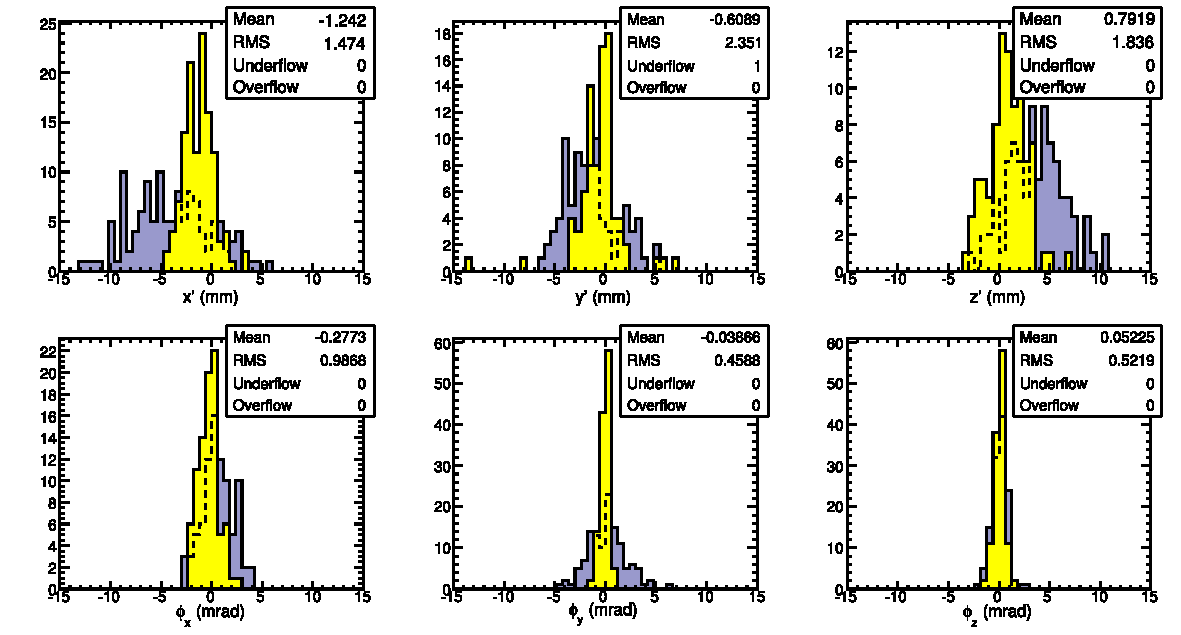
\includegraphics[width=\linewidth]{v4_2008_2009.pdf}
\end{frame}

\begin{frame}
\frametitle{DT alignment}
\begin{center}
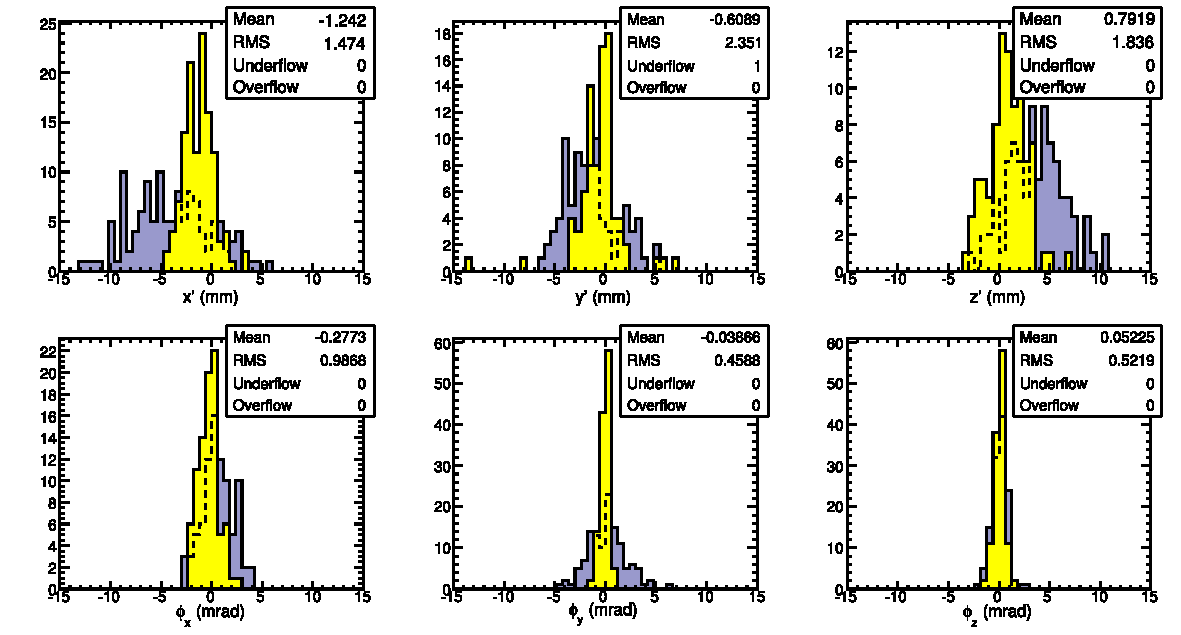
\includegraphics[width=0.8\linewidth]{v4_2008_2009.pdf}
\end{center}
\textcolor{darkblue}{\large Observations:}

\begin{itemize}
\item Angles are reproduced within 0.5~mrad except for $\phi_x$
  (hardest to align; see residuals median studies in CRAFT paper)
\item Translations are on the order of 2~mm, not as large or
  systematic as CRAFT\_ALL\_V4 $\to$ aligned
\item See HyperNews message for details about the sign of the changes
\end{itemize}
\end{frame}

\begin{frame}
\frametitle{DT alignment, split by wheel}

\begin{columns}
\column{0.65\linewidth}
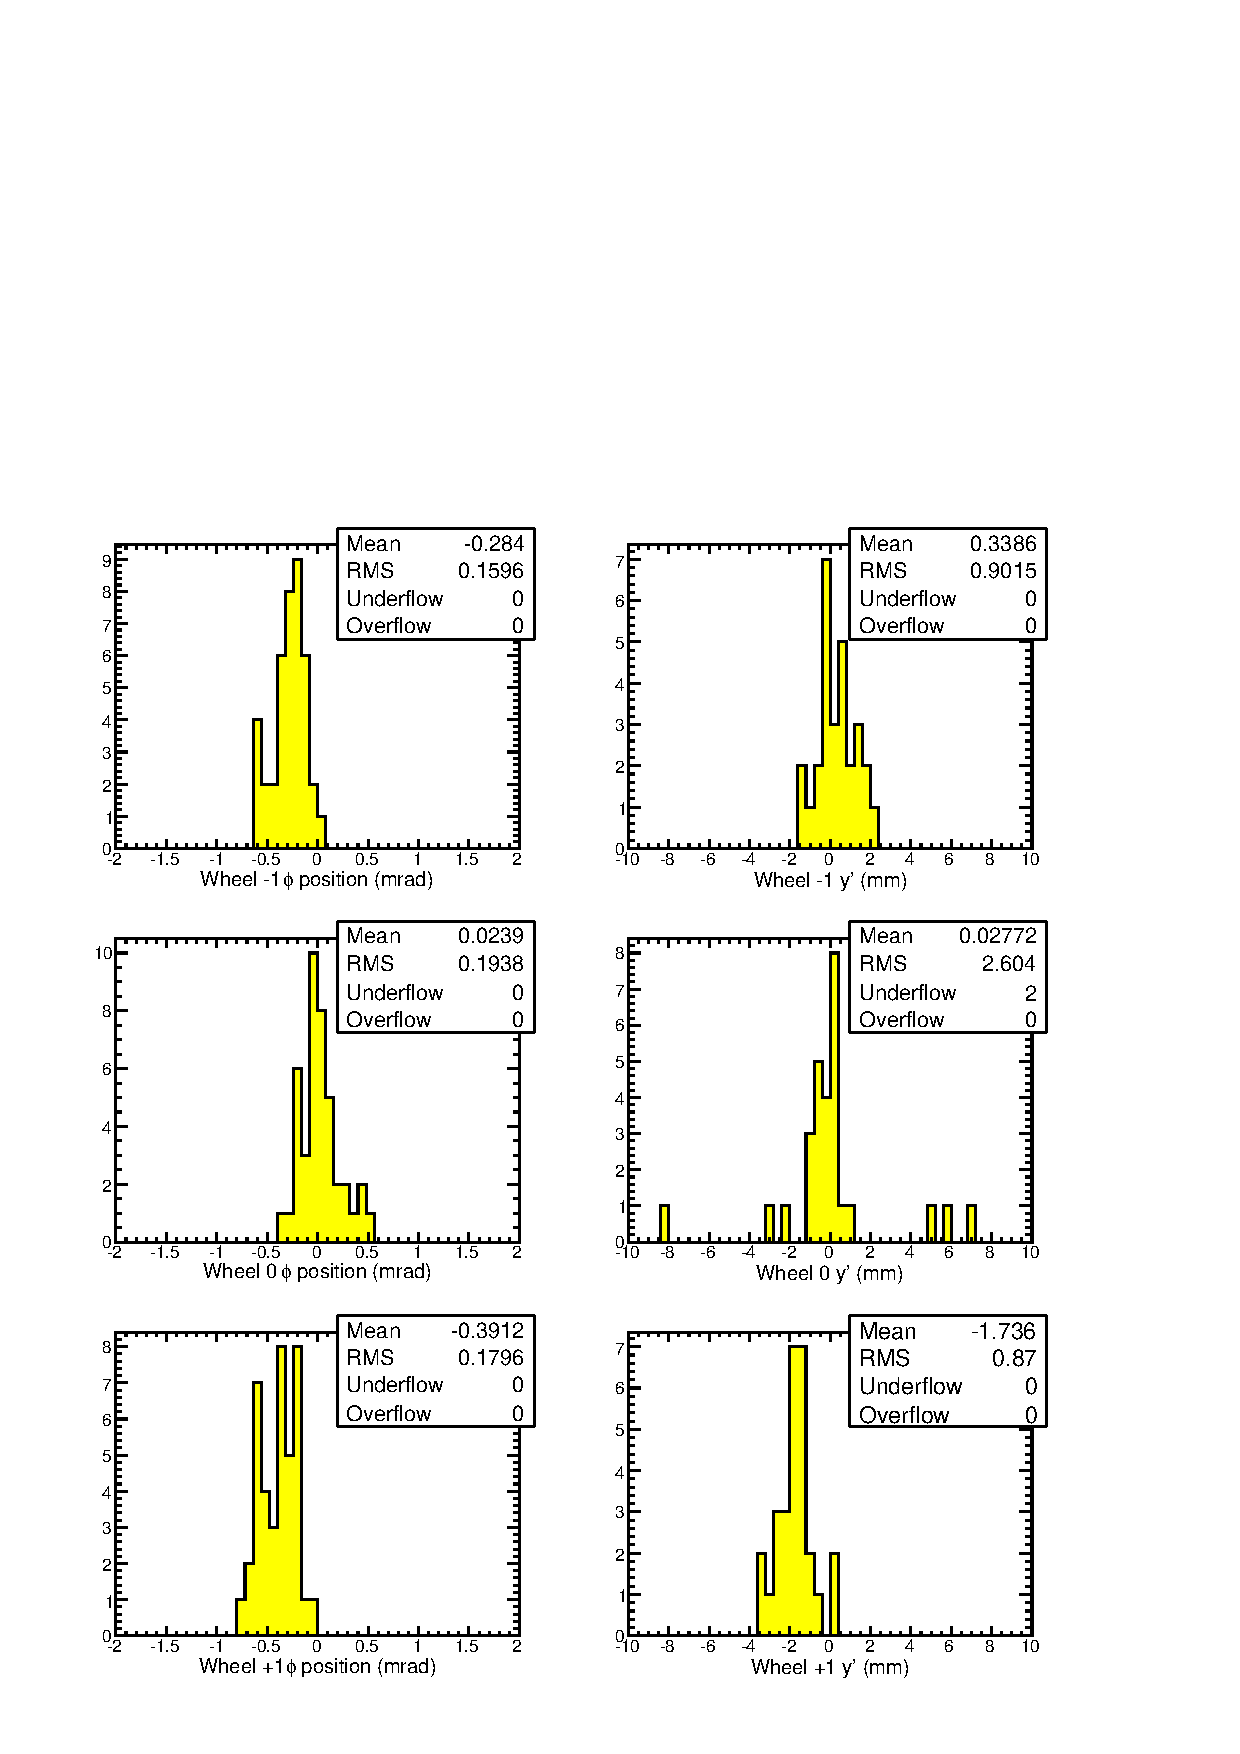
\includegraphics[width=\linewidth]{phipos_yprime_2008_2009.pdf}

\column{0.35\linewidth}
\begin{itemize}
\item Chamber differences are correlated by wheel
\item Wheel~0 seems to be unchanged relative to the tracker (as
  expected)
\item Wheels~$\pm$1 rotated and translated on the order of 0.2~mrad,
  2~mm
\item Large translations parallel to beamline ($y'$) in wheel~0 are
  not yet understood; could be 2008 or 2009 (or real?)
\end{itemize}
\end{columns}
\end{frame}

\begin{frame}
\frametitle{Dependence on tracker}
\begin{itemize}
\item Plots on previous pages maded with 2009 tracker alignment
\item Difference between 2009 muon alignment using (a)~2008 tracker
  and (b)~2009 tracker shown below
\end{itemize}

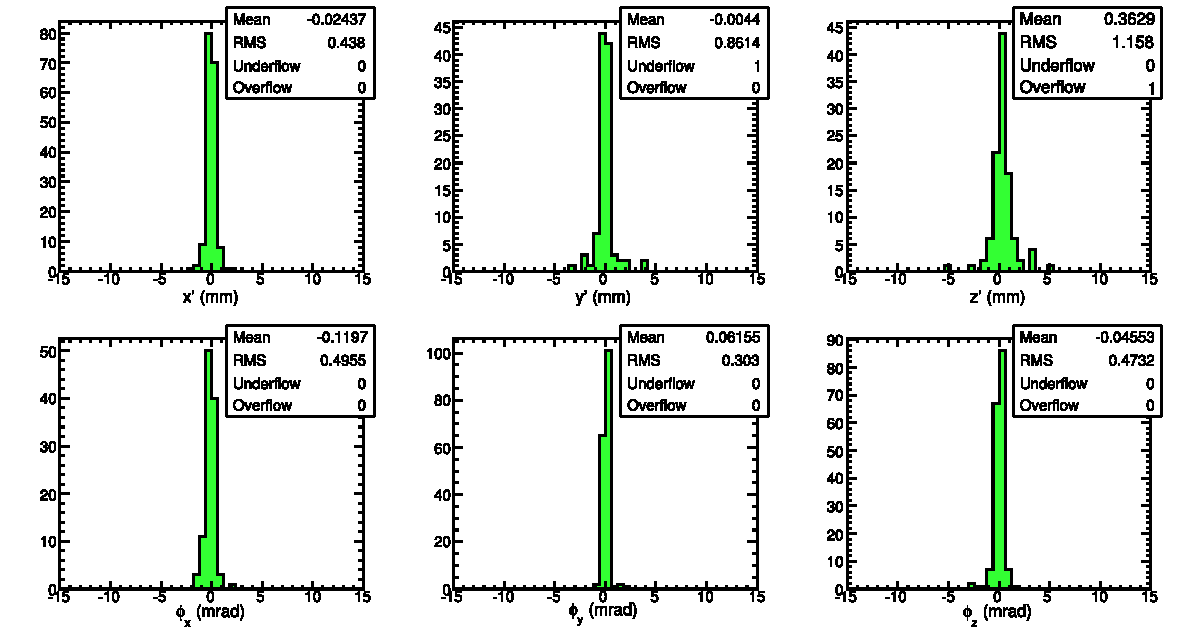
\includegraphics[width=\linewidth]{effect_of_trackeralignment.pdf}
\end{frame}

\begin{frame}
\frametitle{CSC Alignment (method)}

\begin{itemize}
\item Propagate tracks from the tracker to muon chambers \mbox{(same
  as barrel)\hspace{-1 cm}}
\item Compare position and angle of track intersection with segment
  \mbox{(same as barrel, but in $\Delta r\phi$ and $\Delta
  \frac{dr\phi}{dz}$, rather than $\Delta x$, $\Delta y$, $\Delta
  \frac{dx}{dz}$, $\Delta \frac{dy}{dz}$)\hspace{-1 cm}}

{\scriptsize (actually linear-fit of single-hit residuals, to account for possible curvature)}

\item ``$r\phi$'' = direction perpendicular to CSC strips (no granularity)

\item $\Delta r\phi$, $\Delta \frac{d(r\phi)}{dz}$ residuals interpreted as $r\phi$ translation, $\phi_y$ rotation
\end{itemize}

\begin{columns}
\column{0.6\linewidth}
\begin{center}
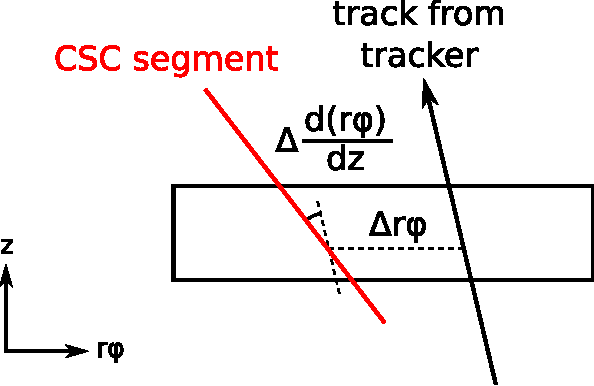
\includegraphics[width=0.7\linewidth]{explanation.pdf}
\end{center}

\column{0.4\linewidth}
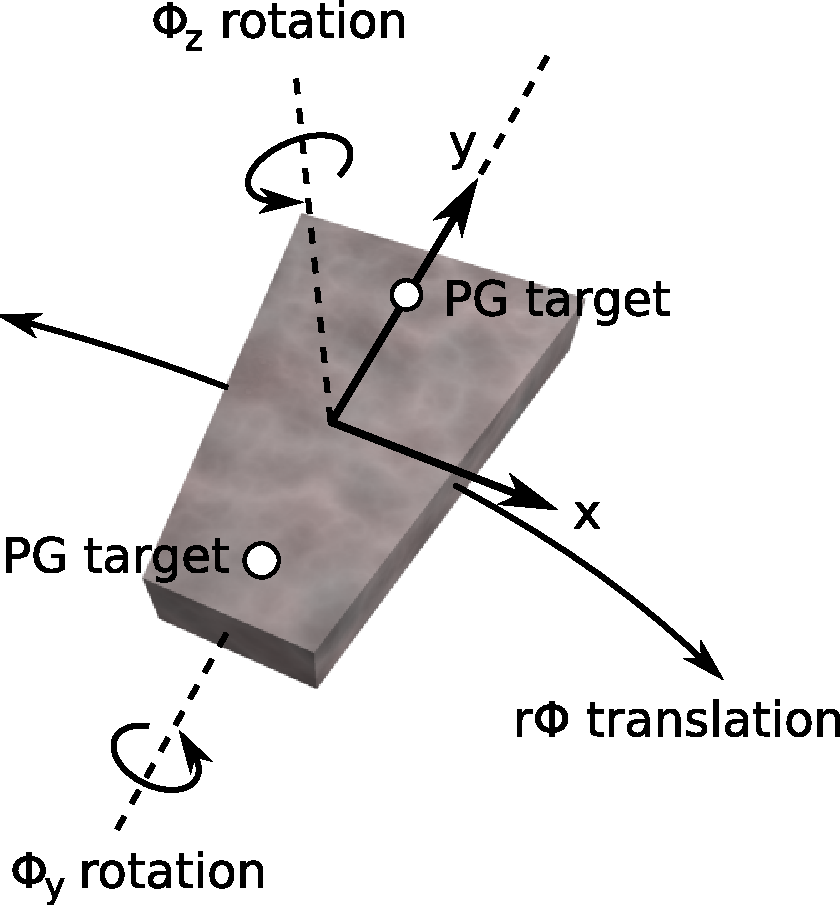
\includegraphics[width=\linewidth]{csc_coordinates.pdf}
\end{columns}
\end{frame}

\begin{frame}
\frametitle{New data are more complete}
\framesubtitle{Chamber angles are independent of disk misalignment}

\vspace{0.2 cm}
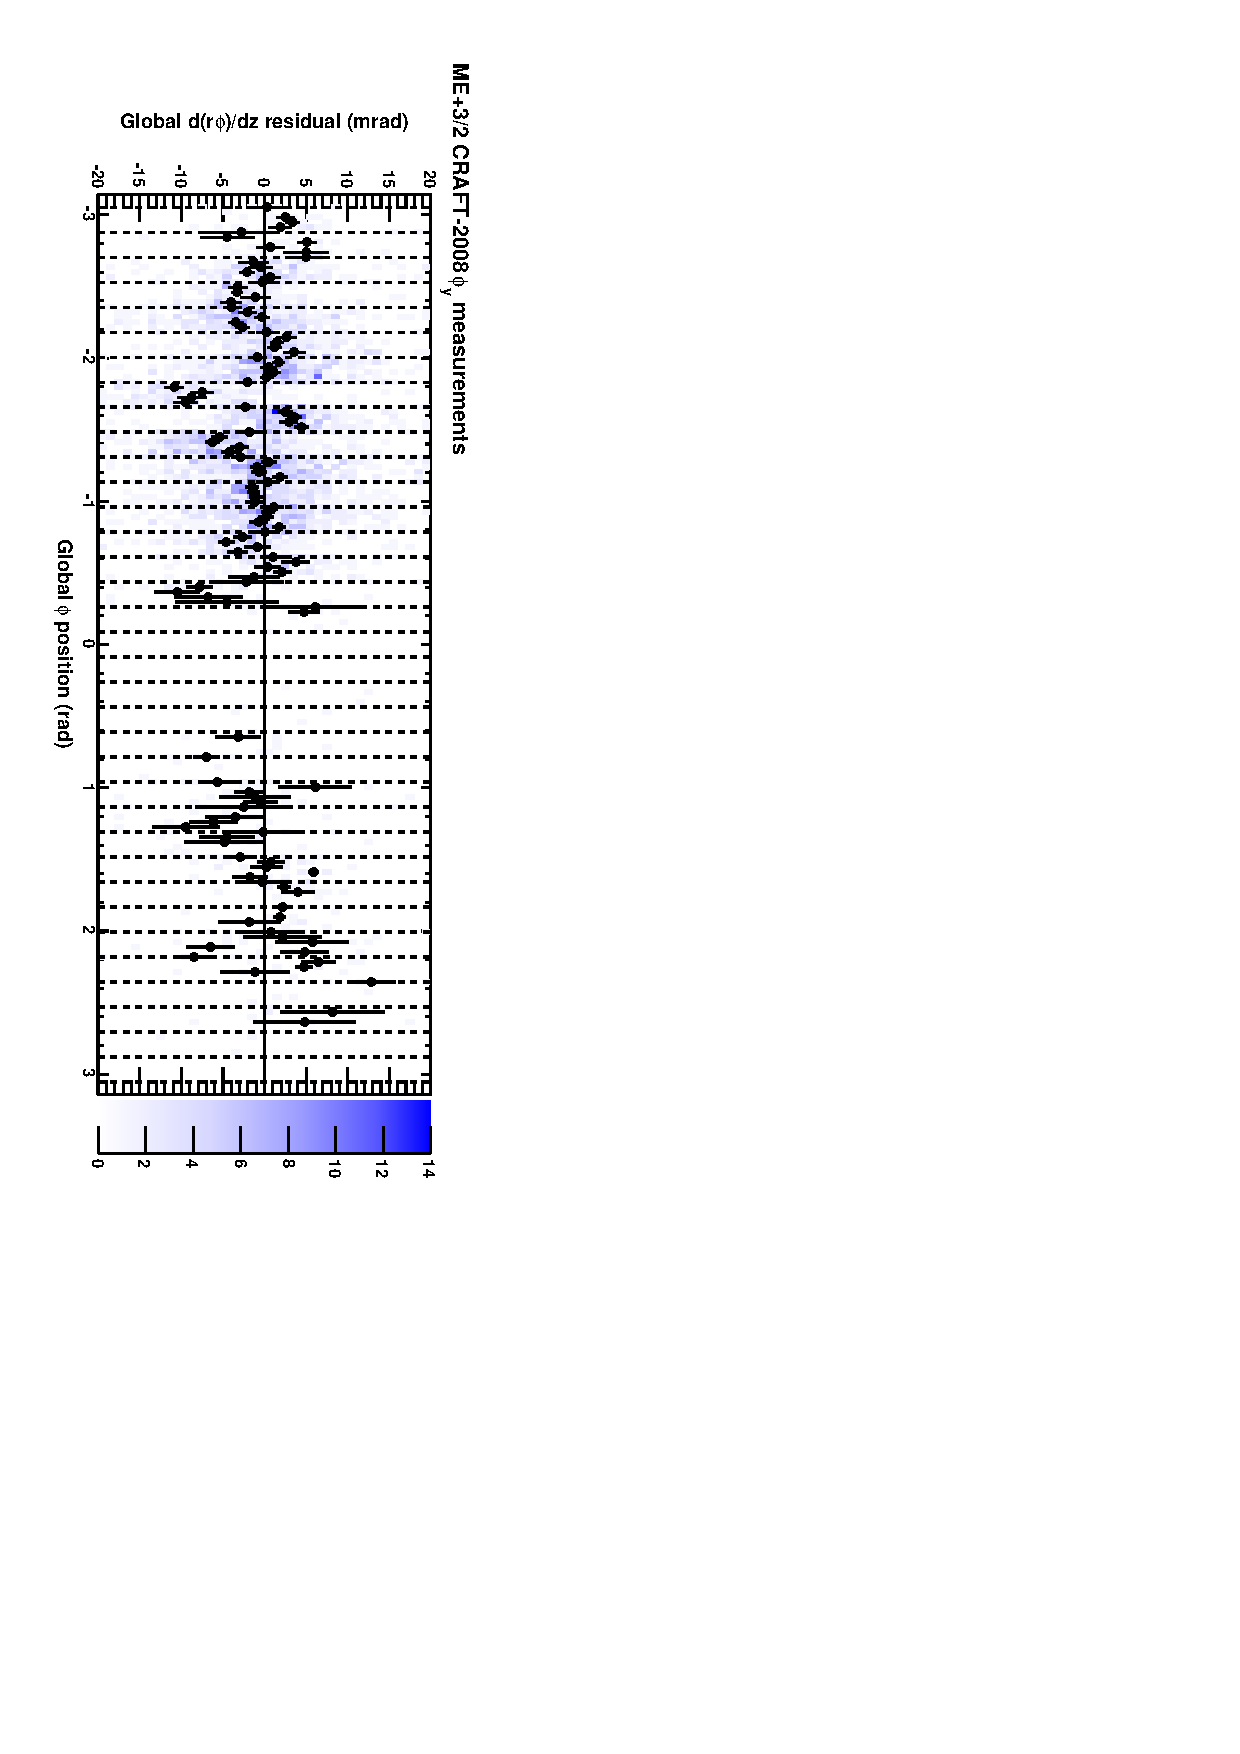
\includegraphics[height=\linewidth, angle=90]{correspondance_2008_mep32_phiy.pdf}

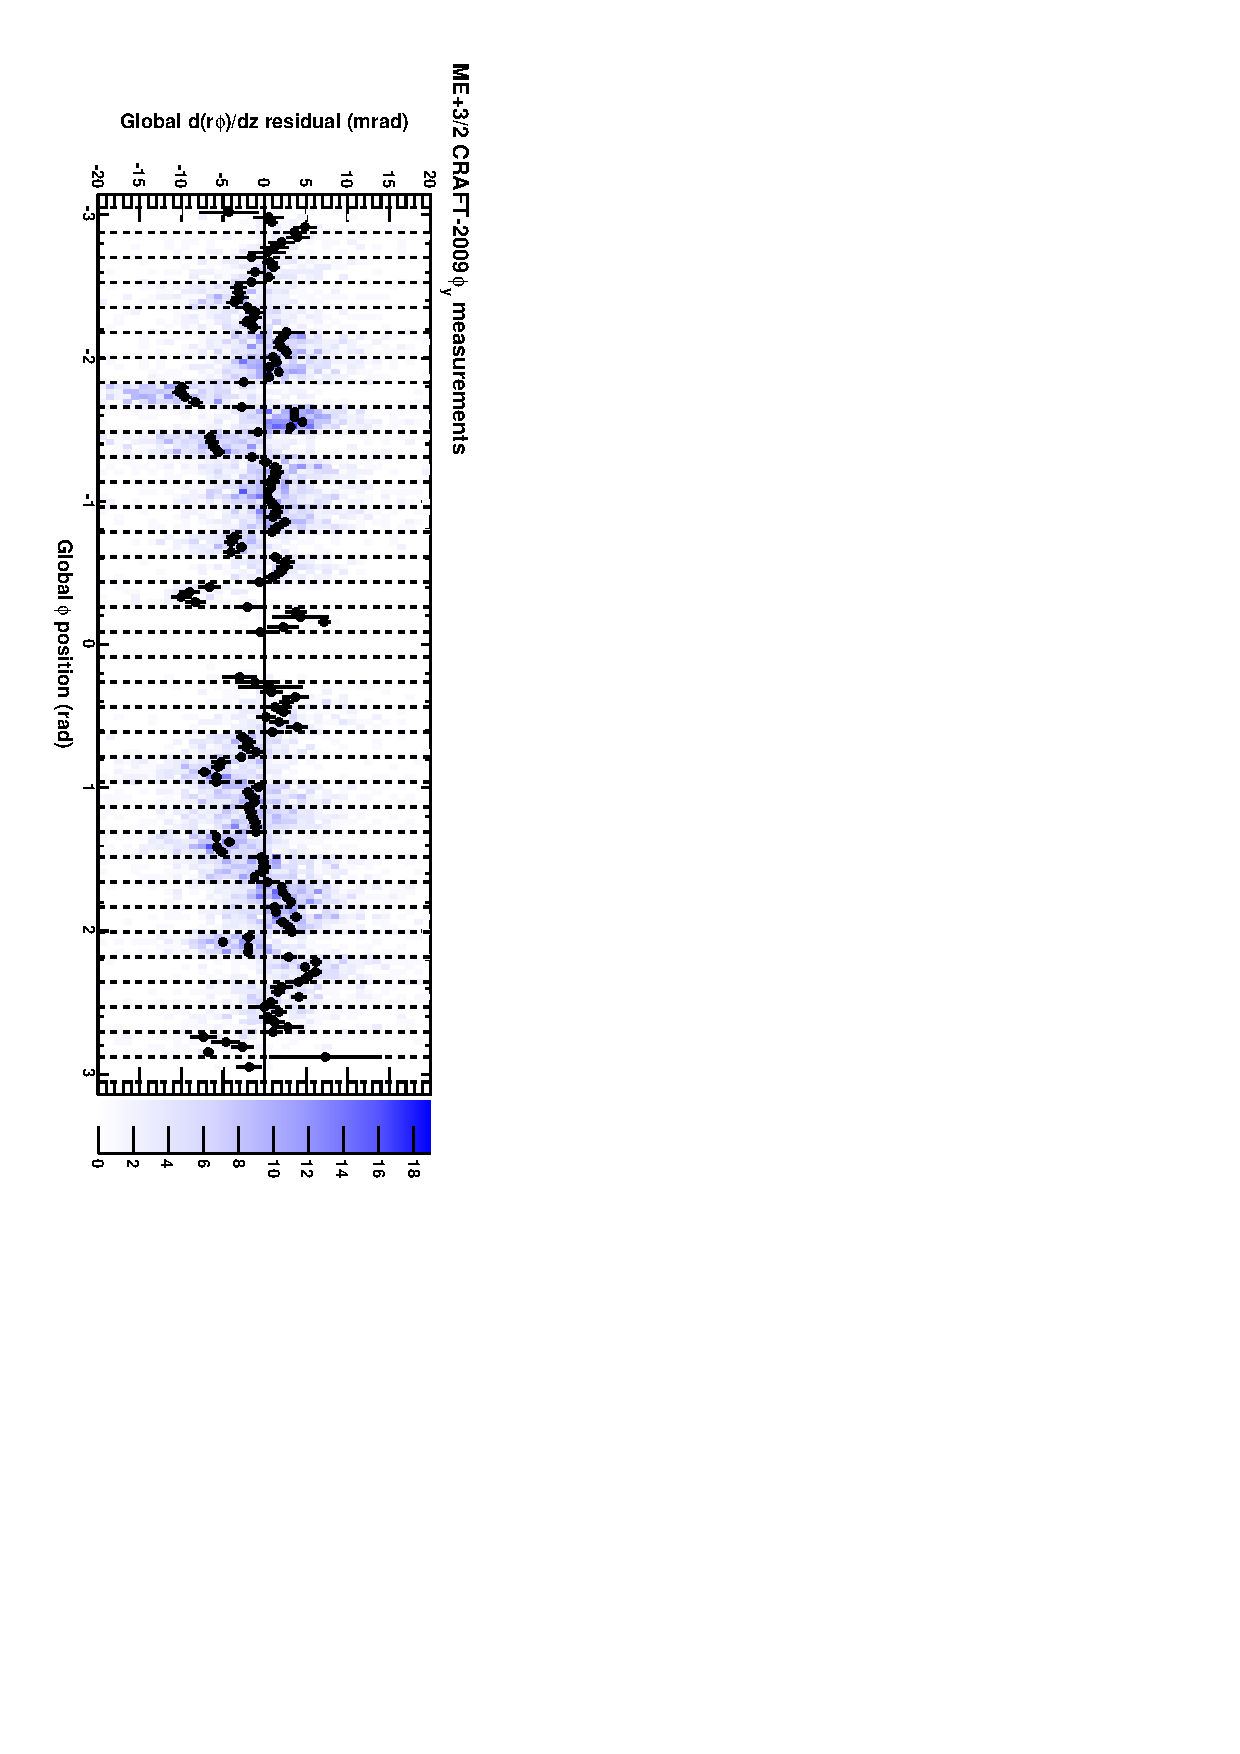
\includegraphics[height=\linewidth, angle=90]{correspondance_2009_mep32_phiy.pdf}
\end{frame}

\begin{frame}
\frametitle{Agreement with beam-halo!}
\framesubtitle{Wider coverage allows us to be sure that the correlation is real}

\vspace{0.2 cm}
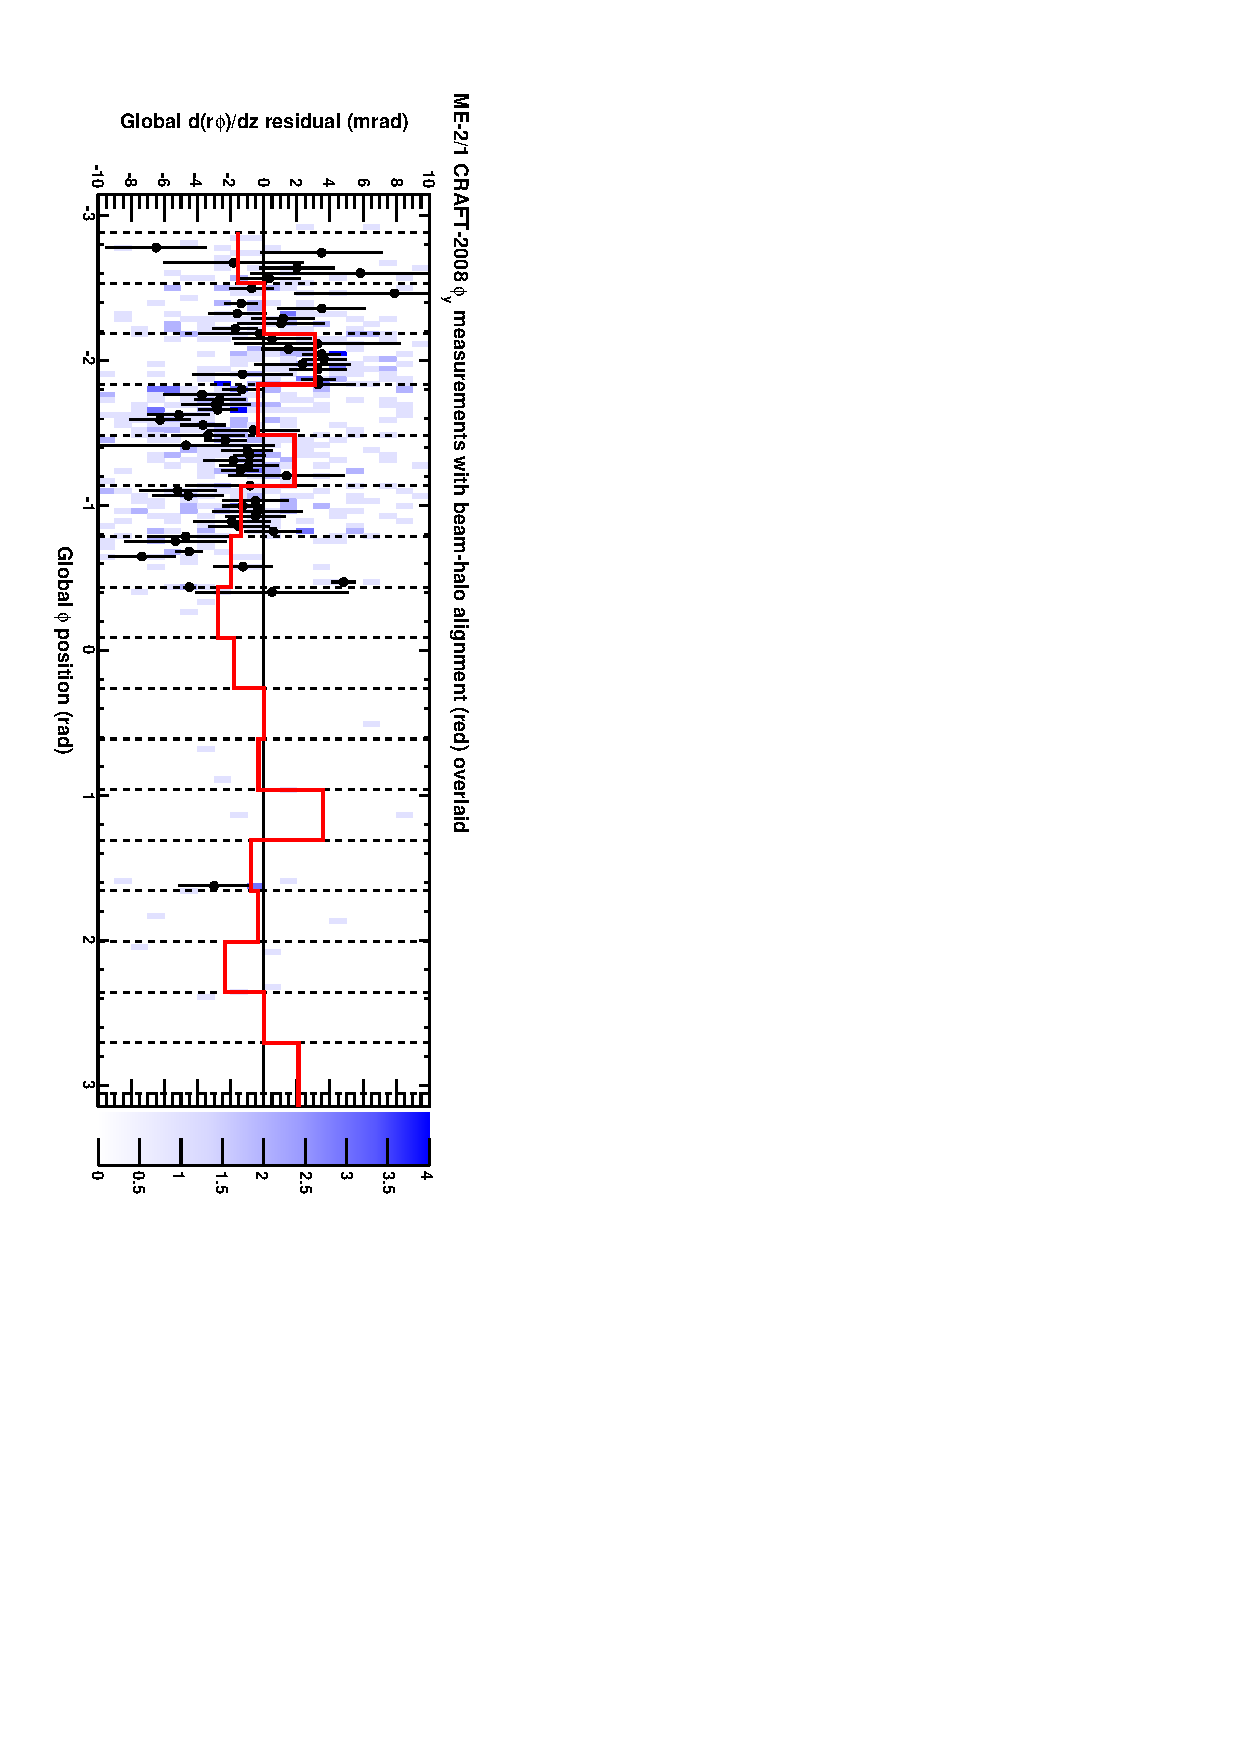
\includegraphics[height=\linewidth, angle=90]{beamhalo_2008_mem21.pdf}

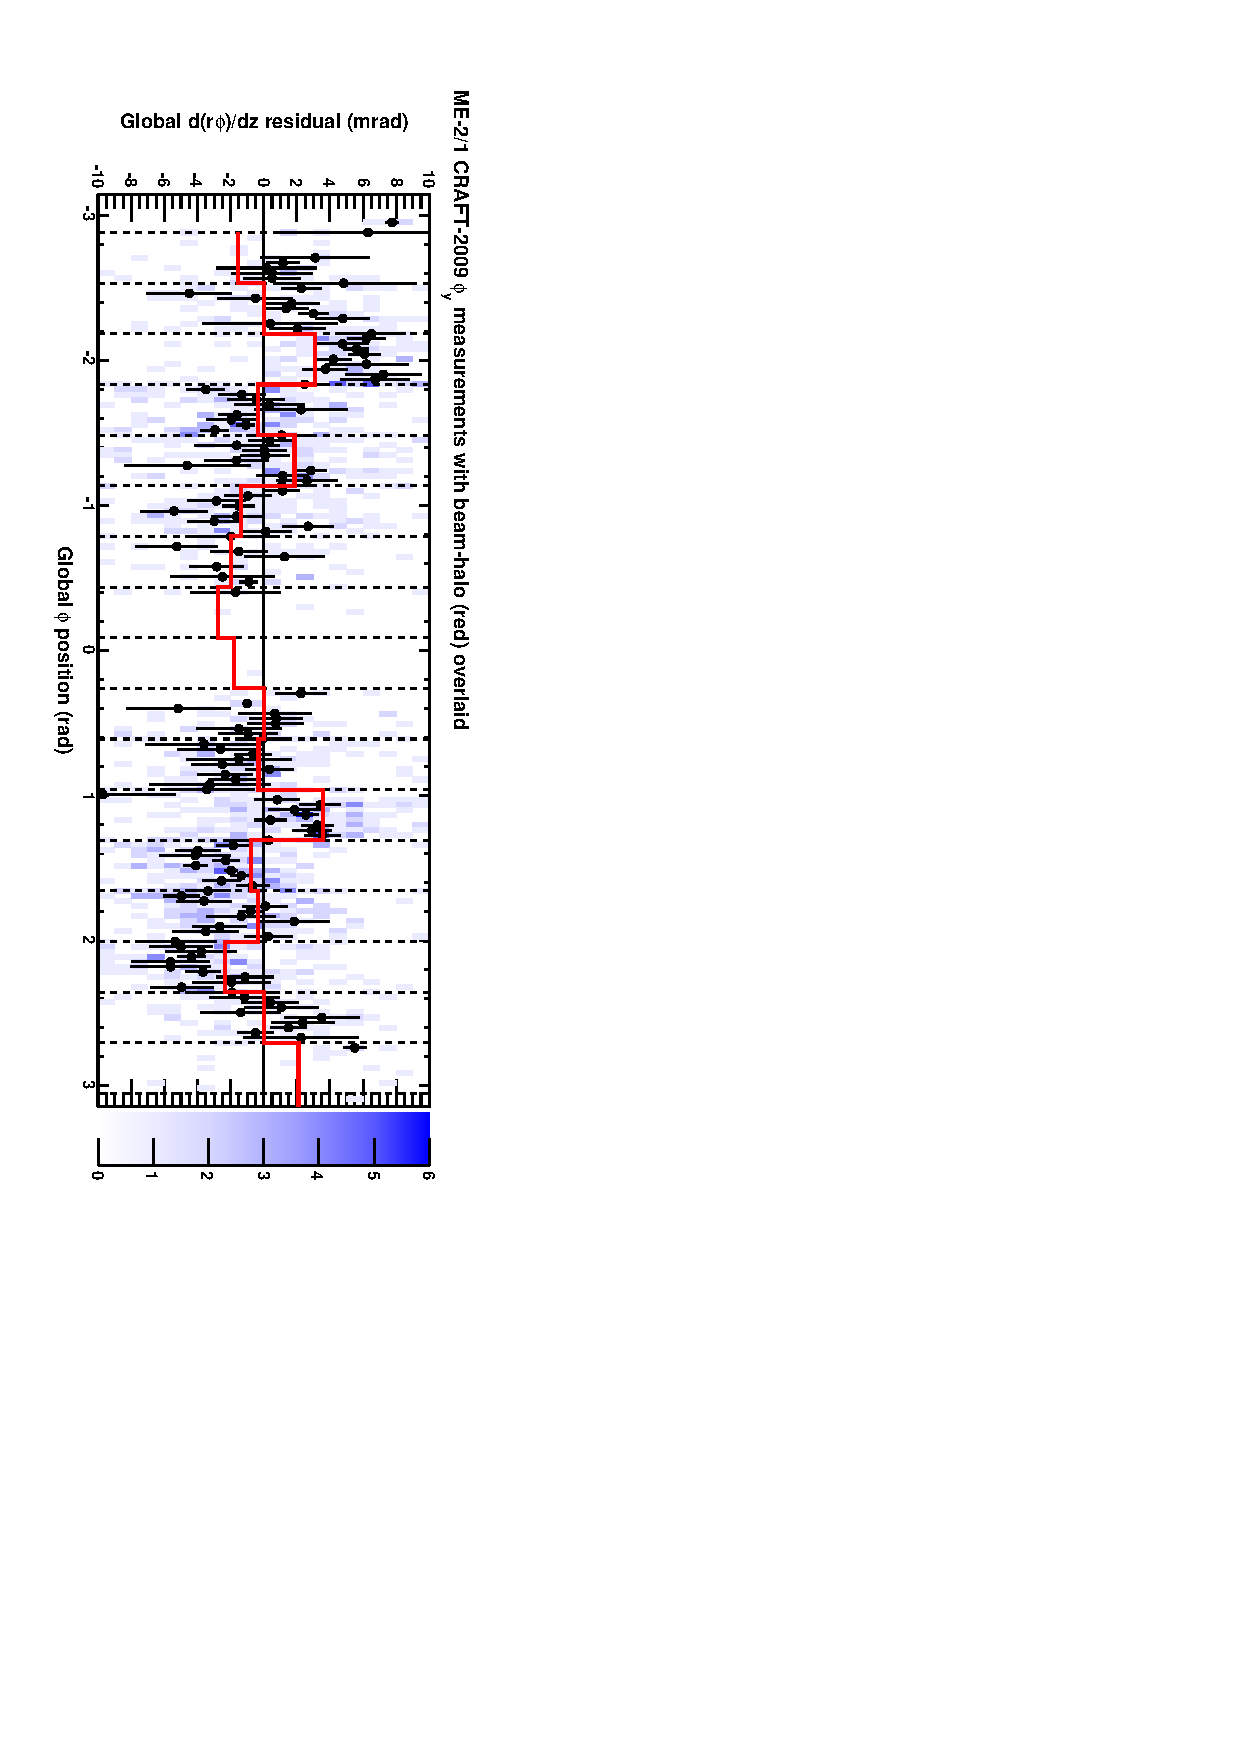
\includegraphics[height=\linewidth, angle=90]{beamhalo_2009_mem21.pdf}
\end{frame}

\begin{frame}
\frametitle{Agreement with beam-halo?}
\framesubtitle{But there are some significant differences: likely real motion}

\vspace{0.2 cm}
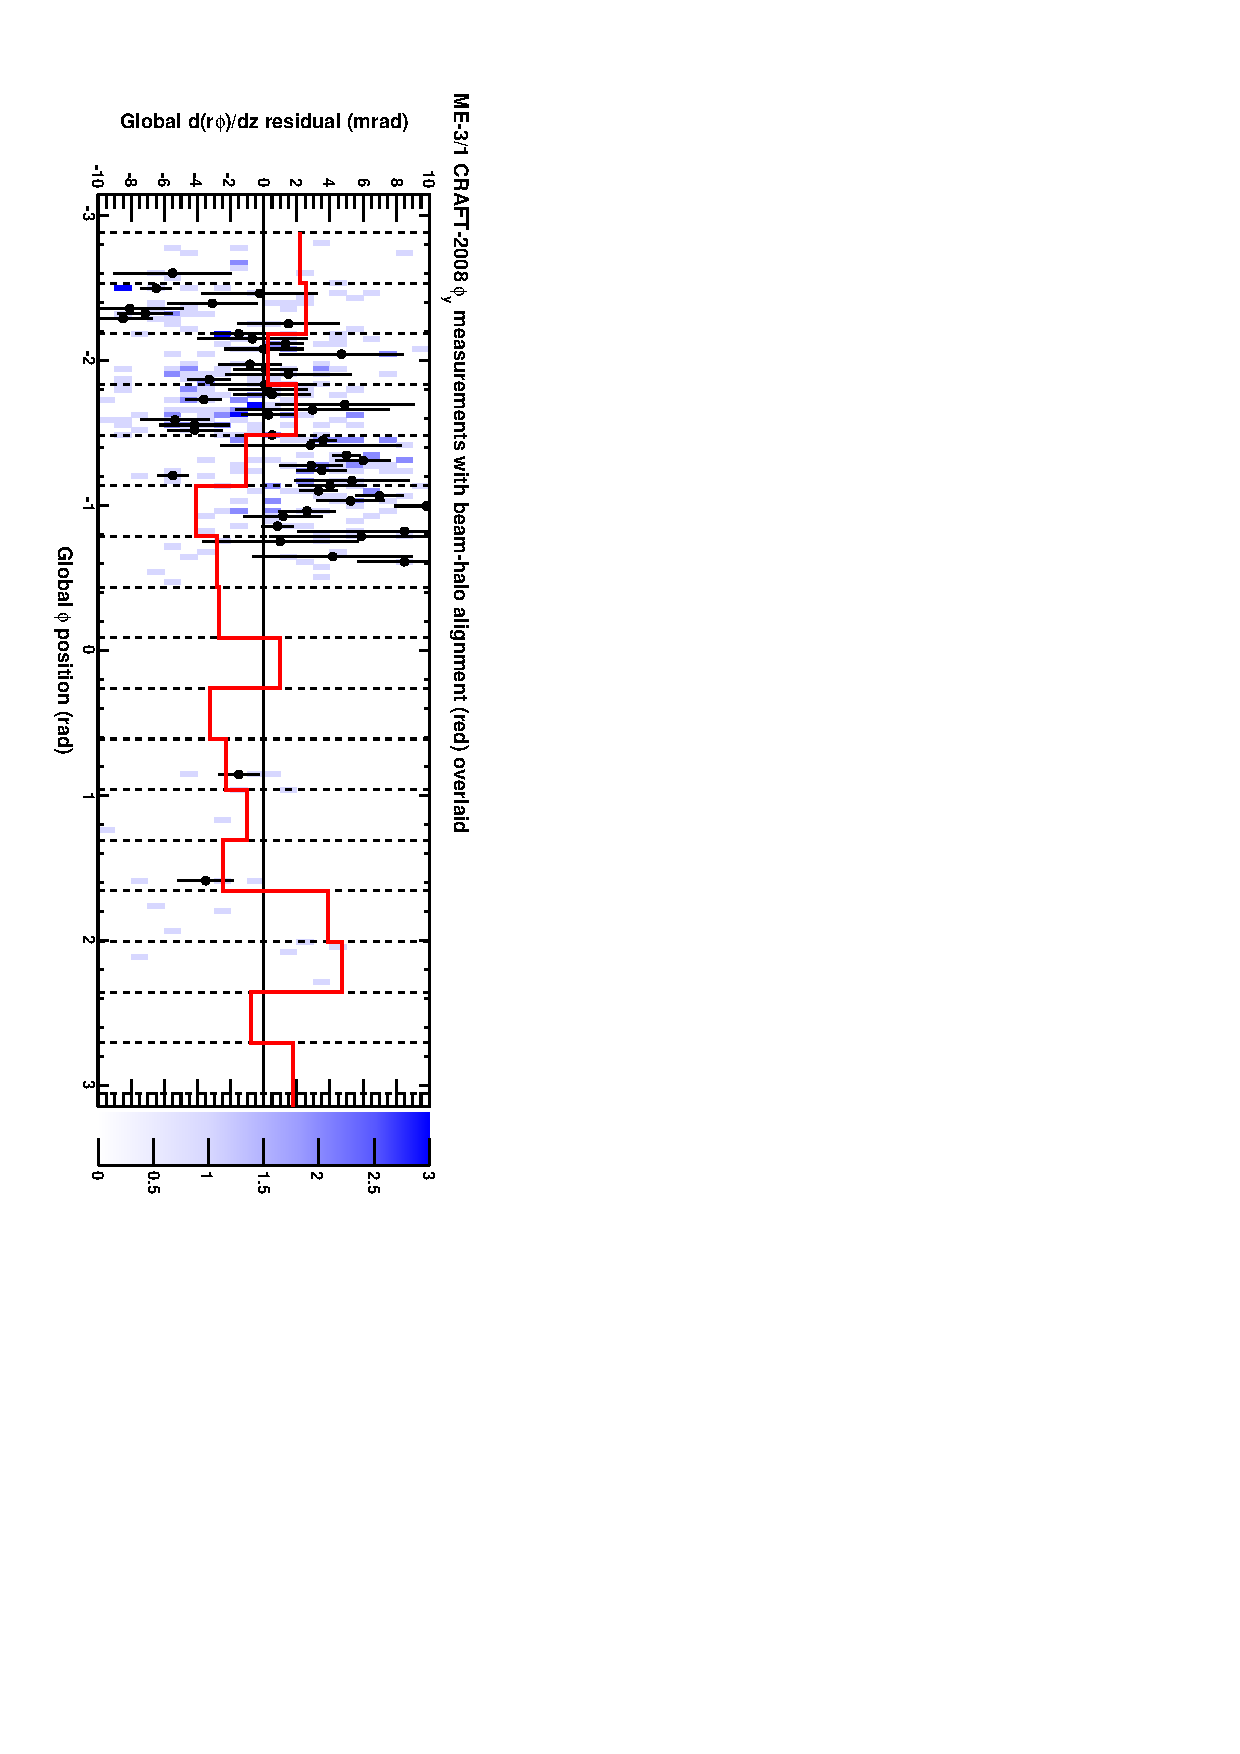
\includegraphics[height=\linewidth, angle=90]{beamhalo_2008_mem31.pdf}

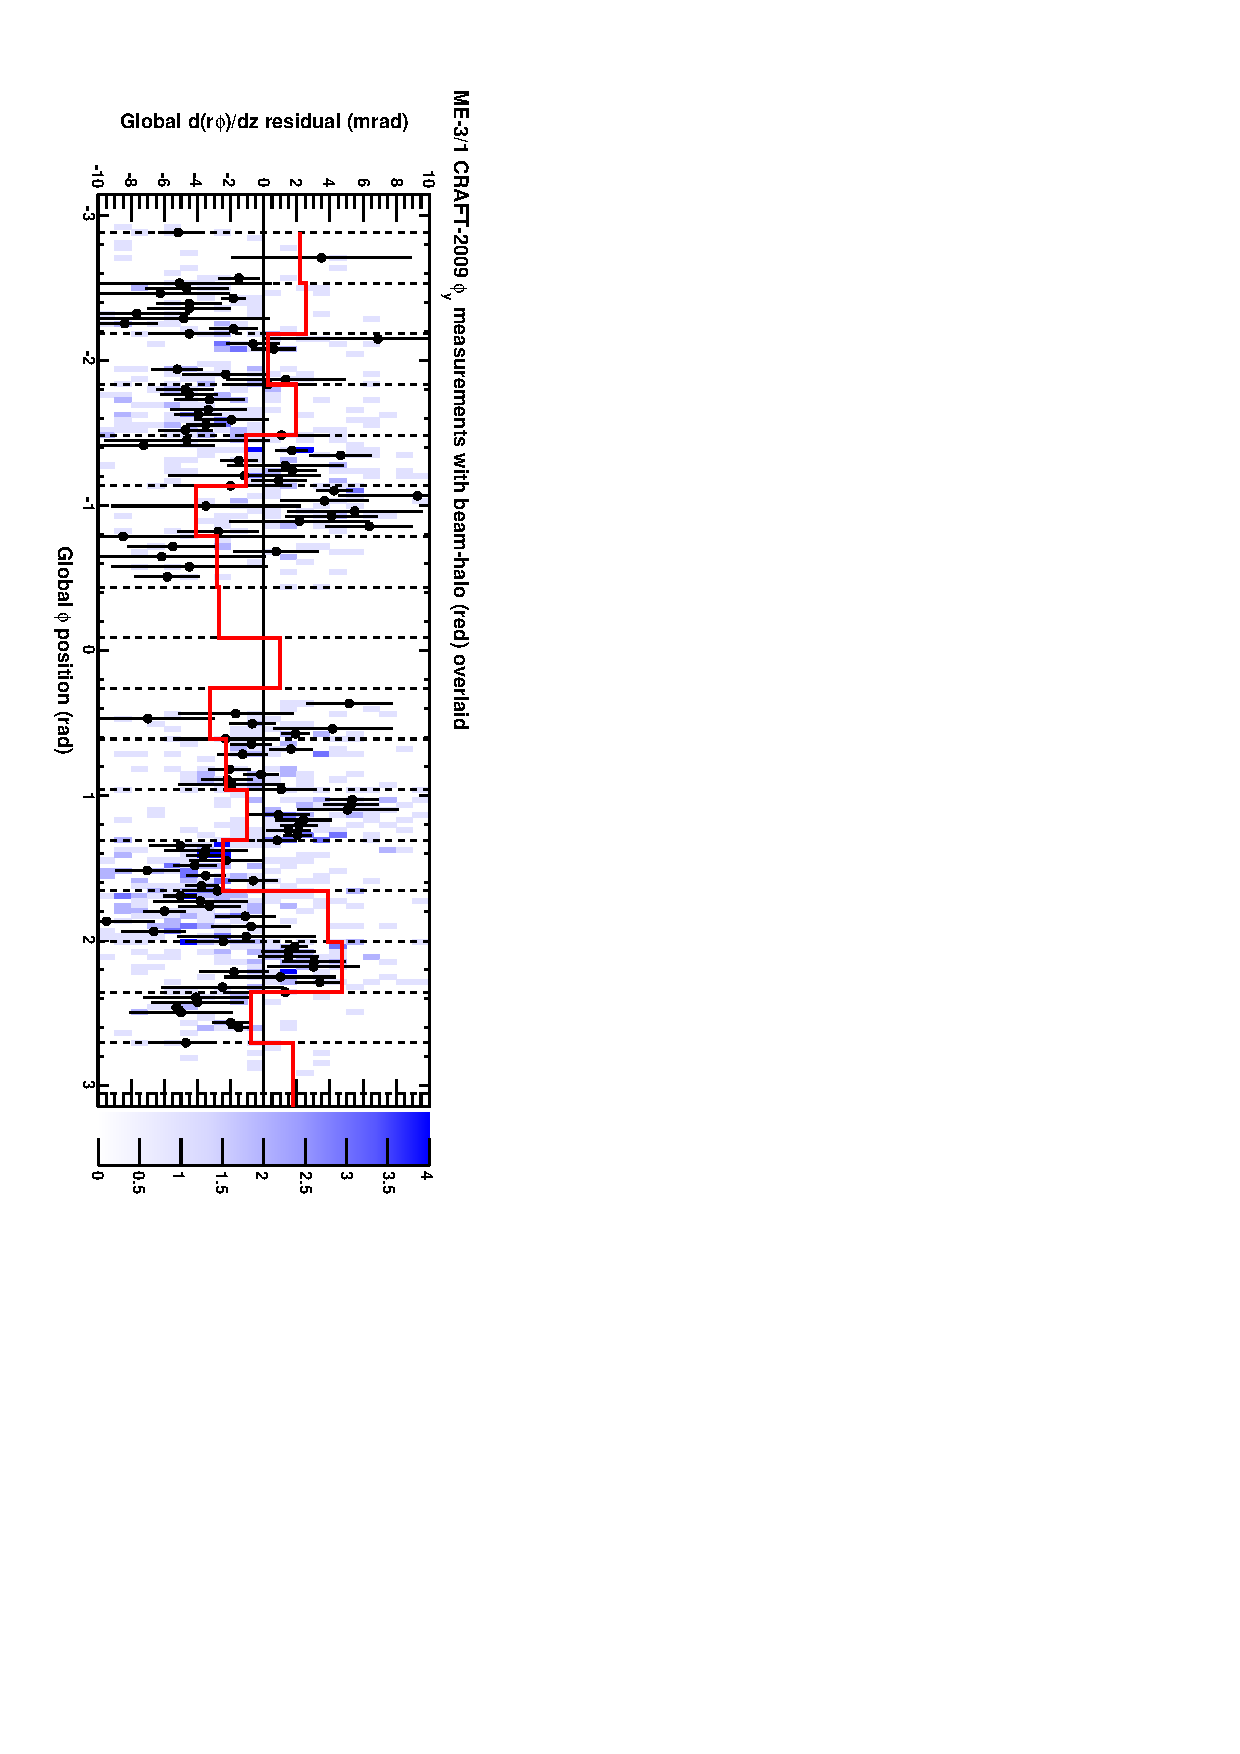
\includegraphics[height=\linewidth, angle=90]{beamhalo_2009_mem31.pdf}
\end{frame}

\begin{frame}
\frametitle{Discontinuities at boundaries}
\framesubtitle{Reminder of an argument about the interpretation of
  residuals vs.~$\phi$ plots}

\begin{center}
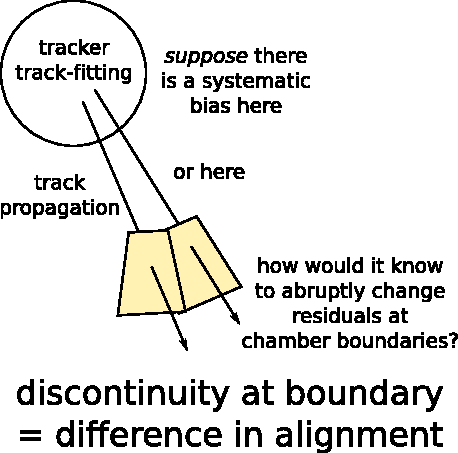
\includegraphics[width=0.55\linewidth]{argument.pdf}
\end{center}

\large \ldots or something else related to the chambers themselves, not the track source
\end{frame}

\begin{frame}
\frametitle{$\Delta r\phi$ position residuals}
\framesubtitle{Nicely completed $(\mbox{const} + \sin\phi + \cos\phi)$ curve, but why the alteration?}

\vspace{0.2 cm}
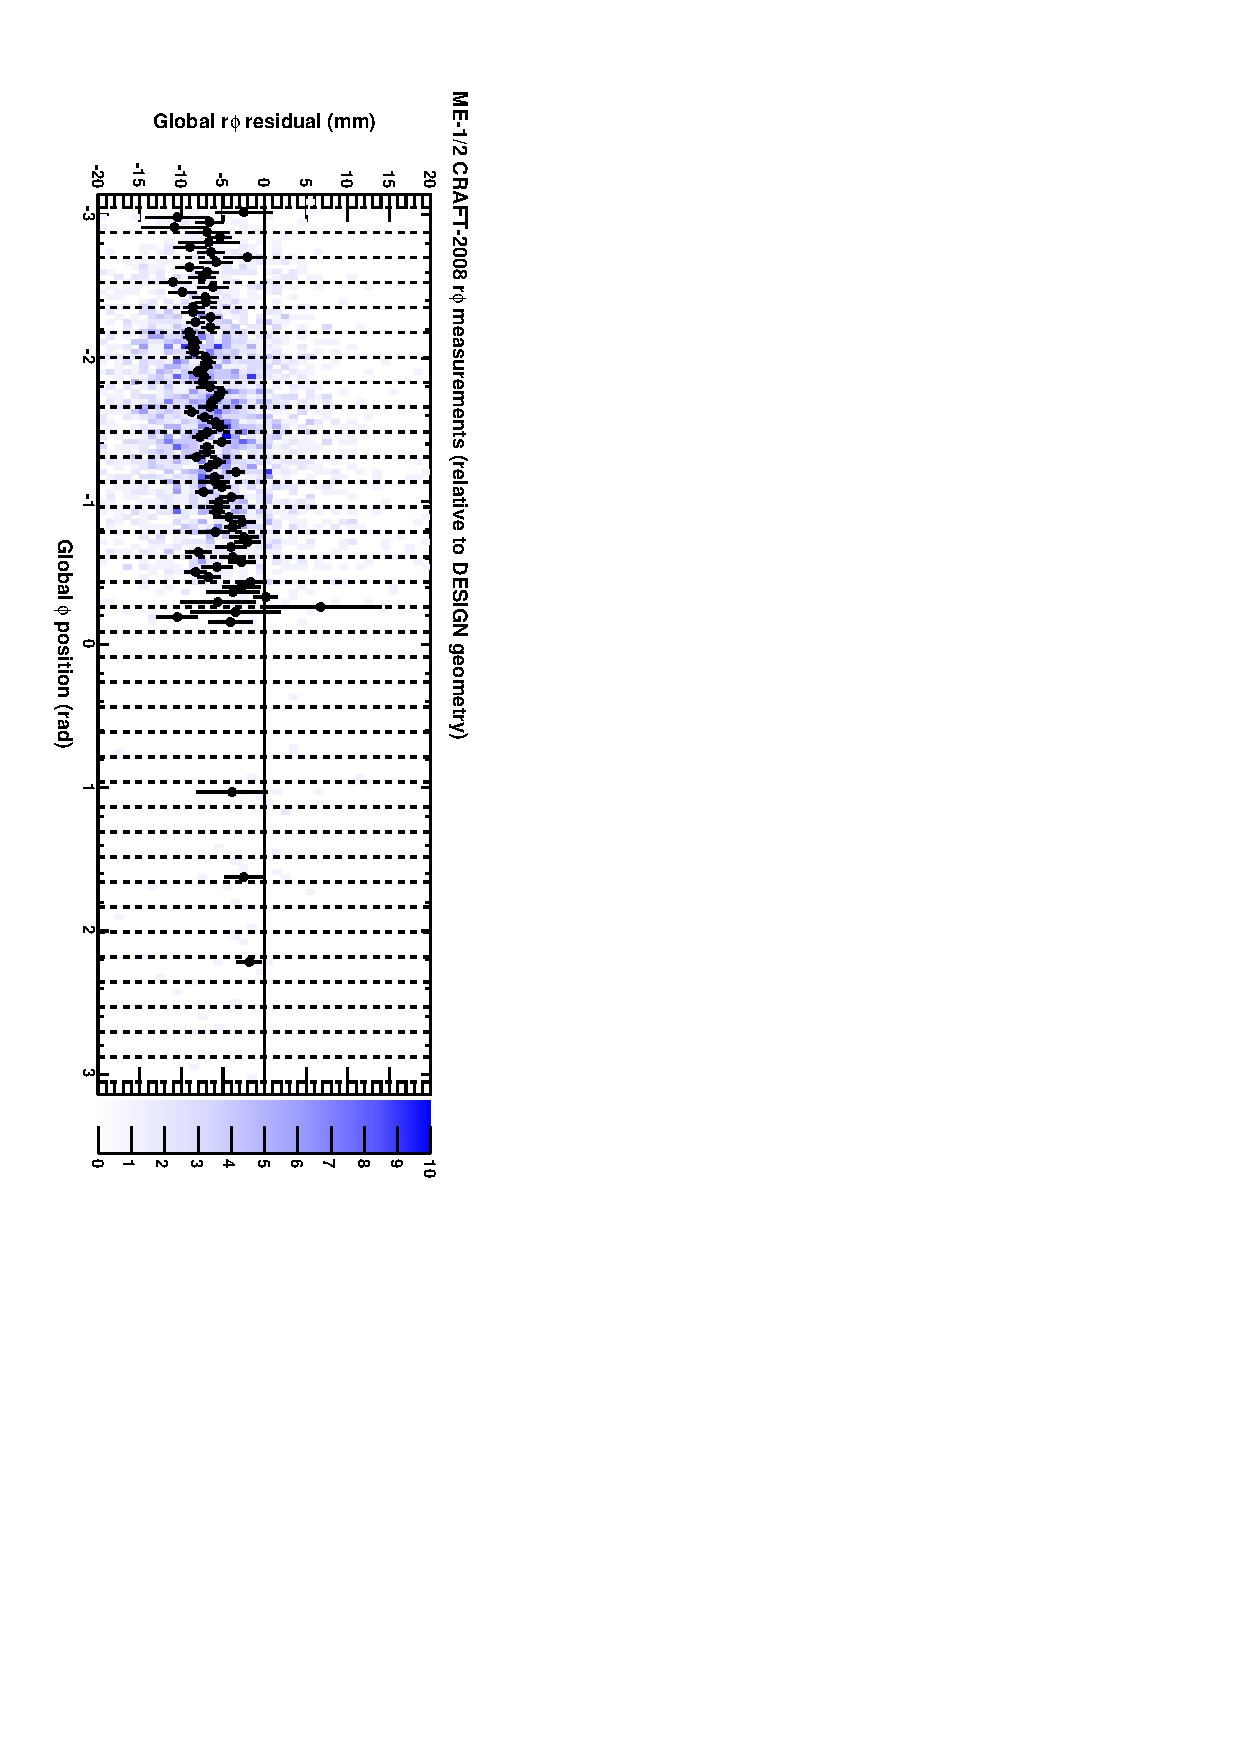
\includegraphics[height=\linewidth, angle=90]{alternation_2008_mem12_design.pdf}

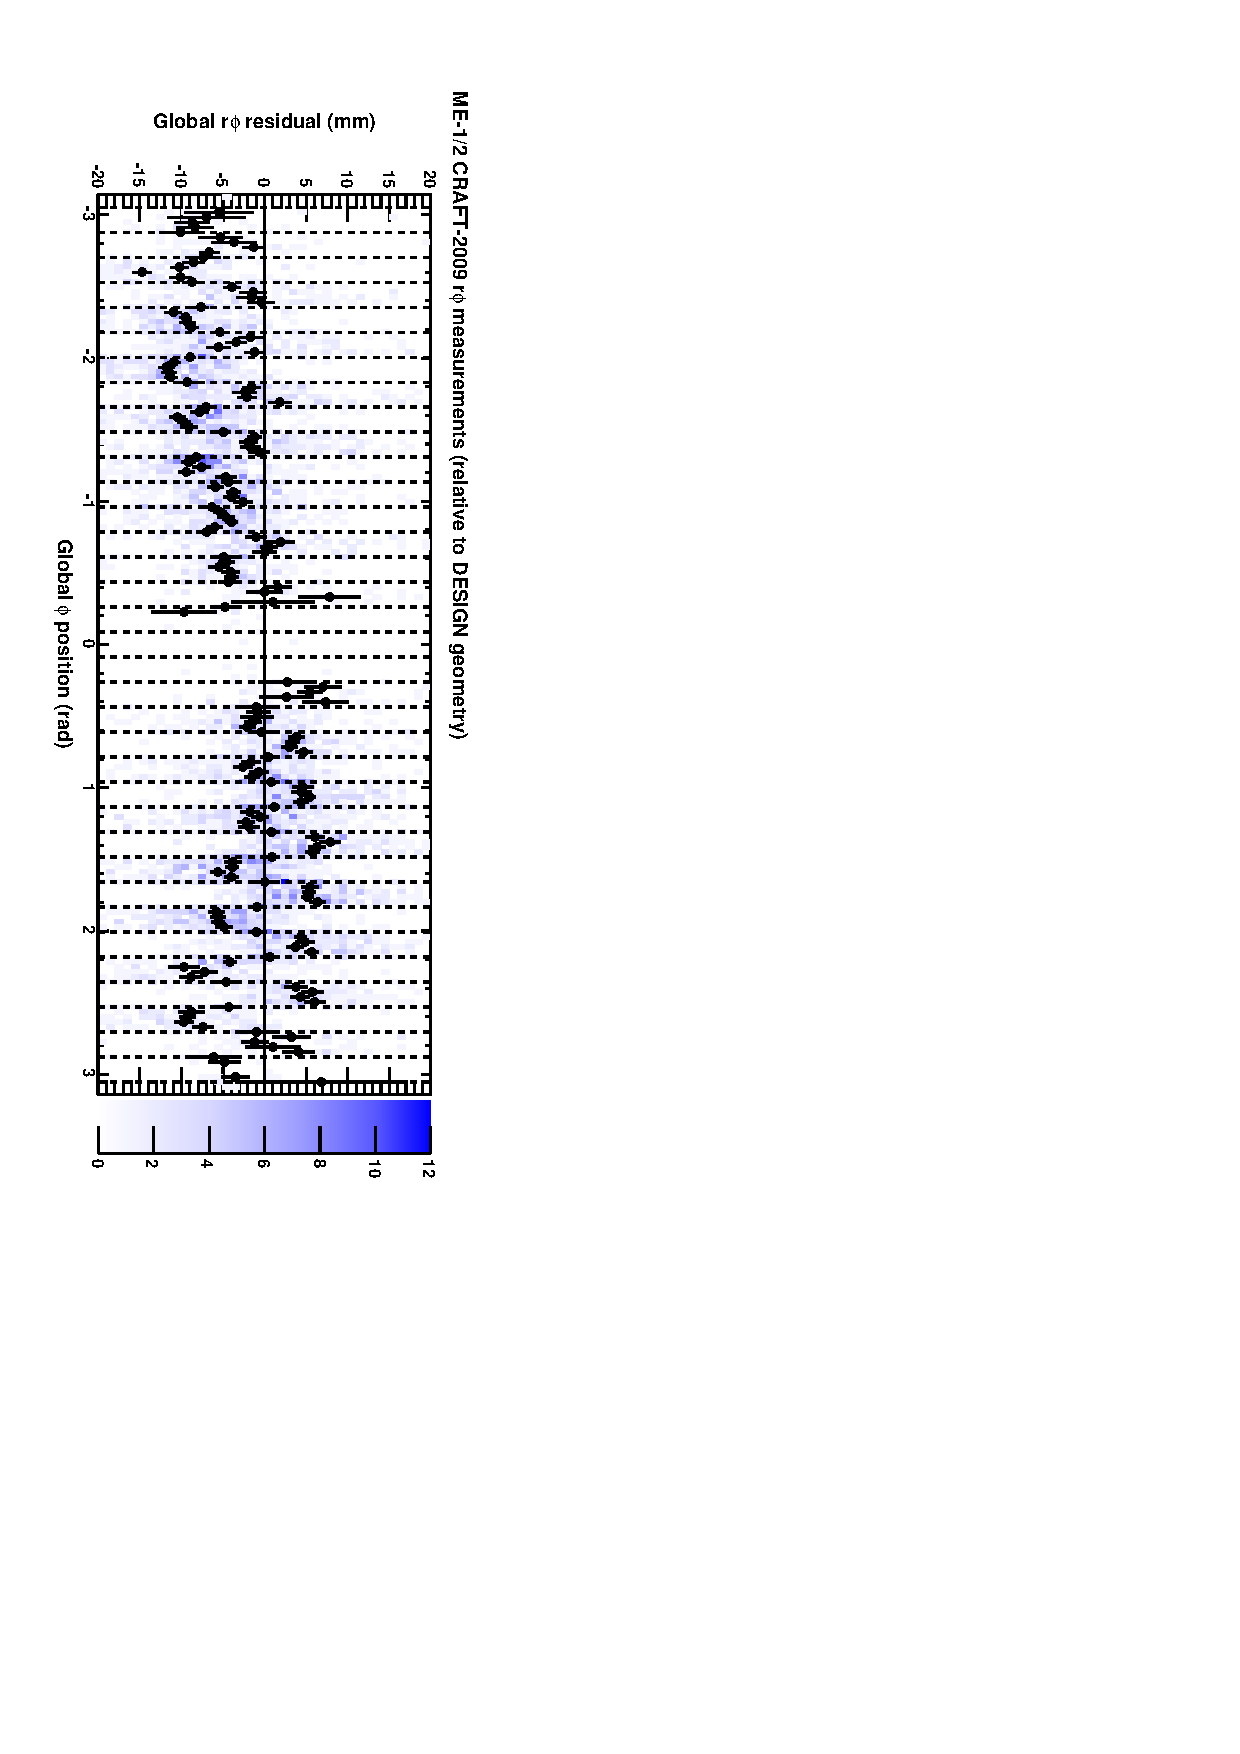
\includegraphics[height=\linewidth, angle=90]{alternation_2009_mem12_design.pdf}
\end{frame}

\begin{frame}
\frametitle{Now with HW/PG geometry\ldots}
\framesubtitle{Also insensitive to a 1~cm translation in $z$}

\vspace{0.2 cm}
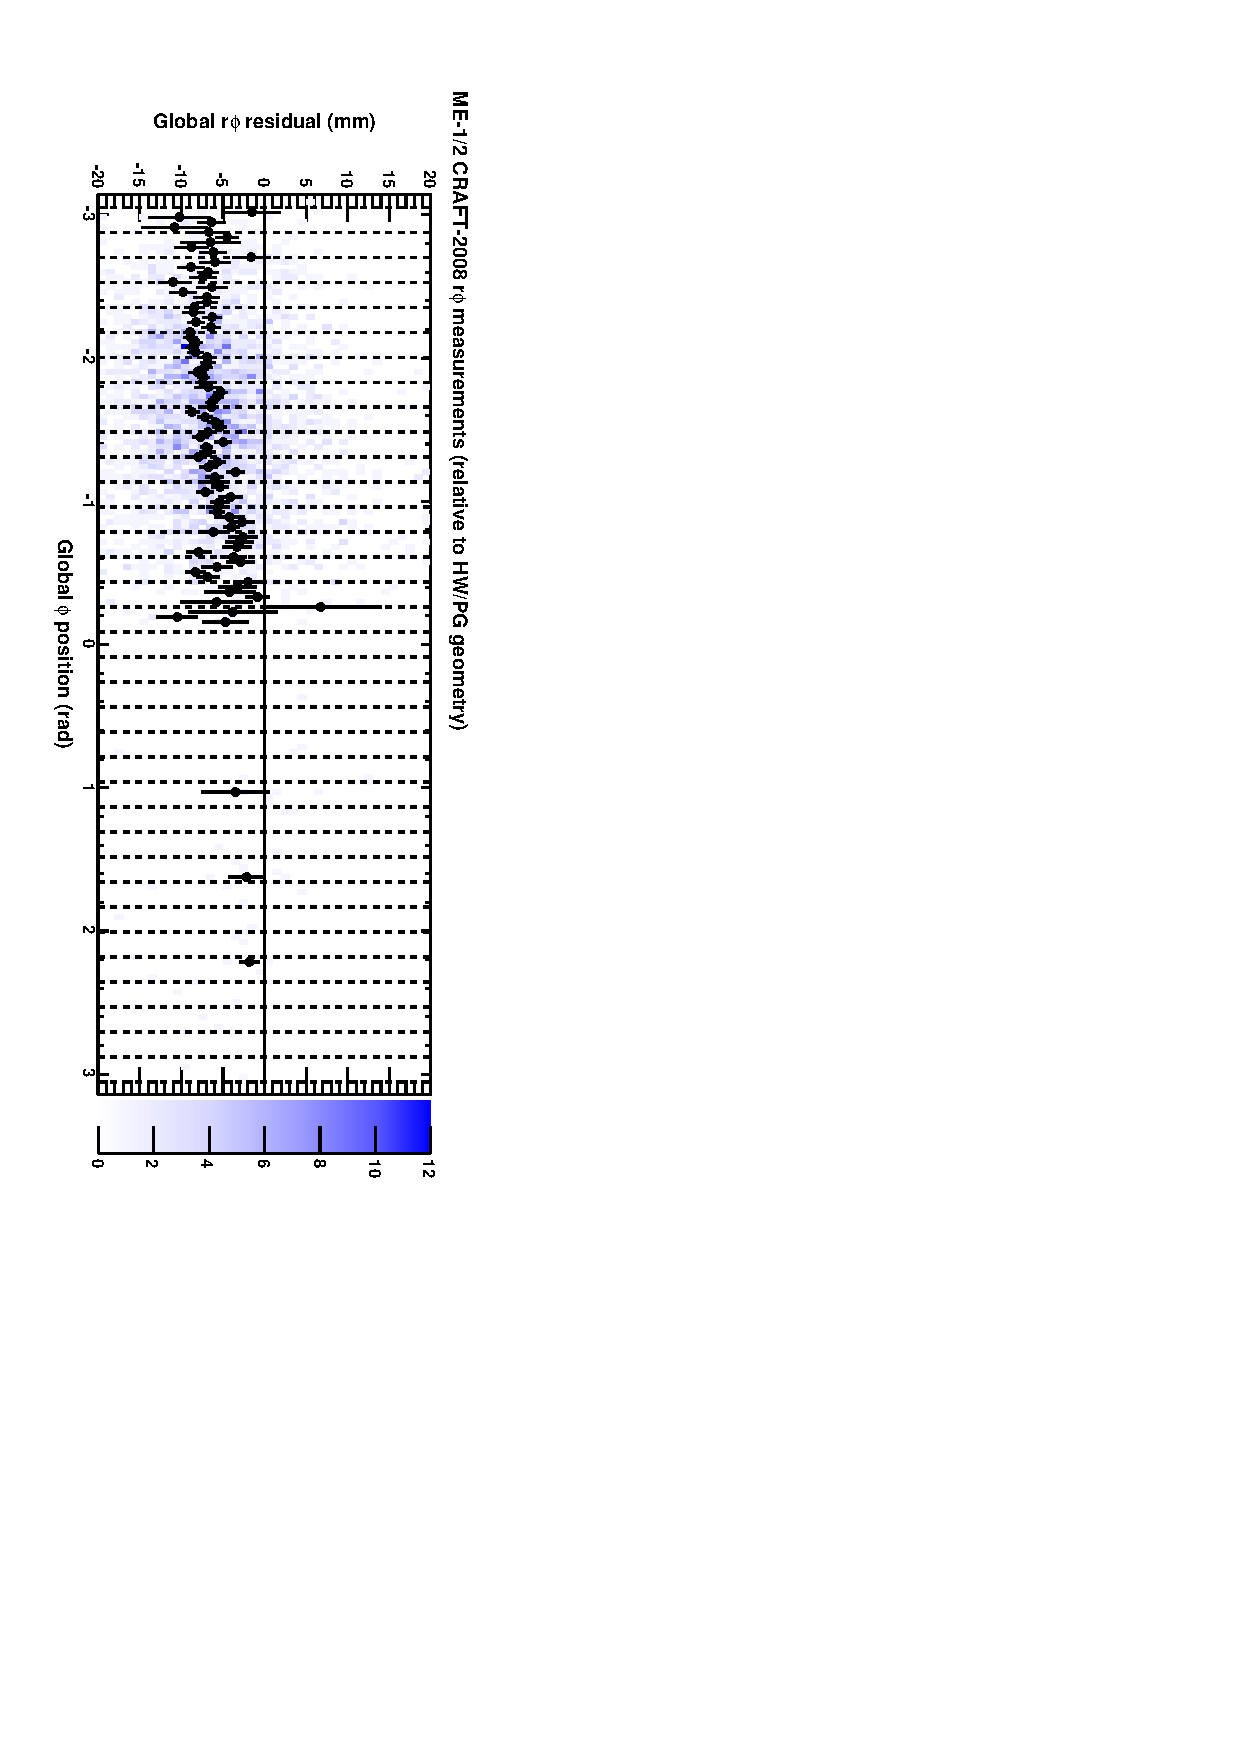
\includegraphics[height=\linewidth, angle=90]{alternation_2008_mem12_hwpg.pdf}

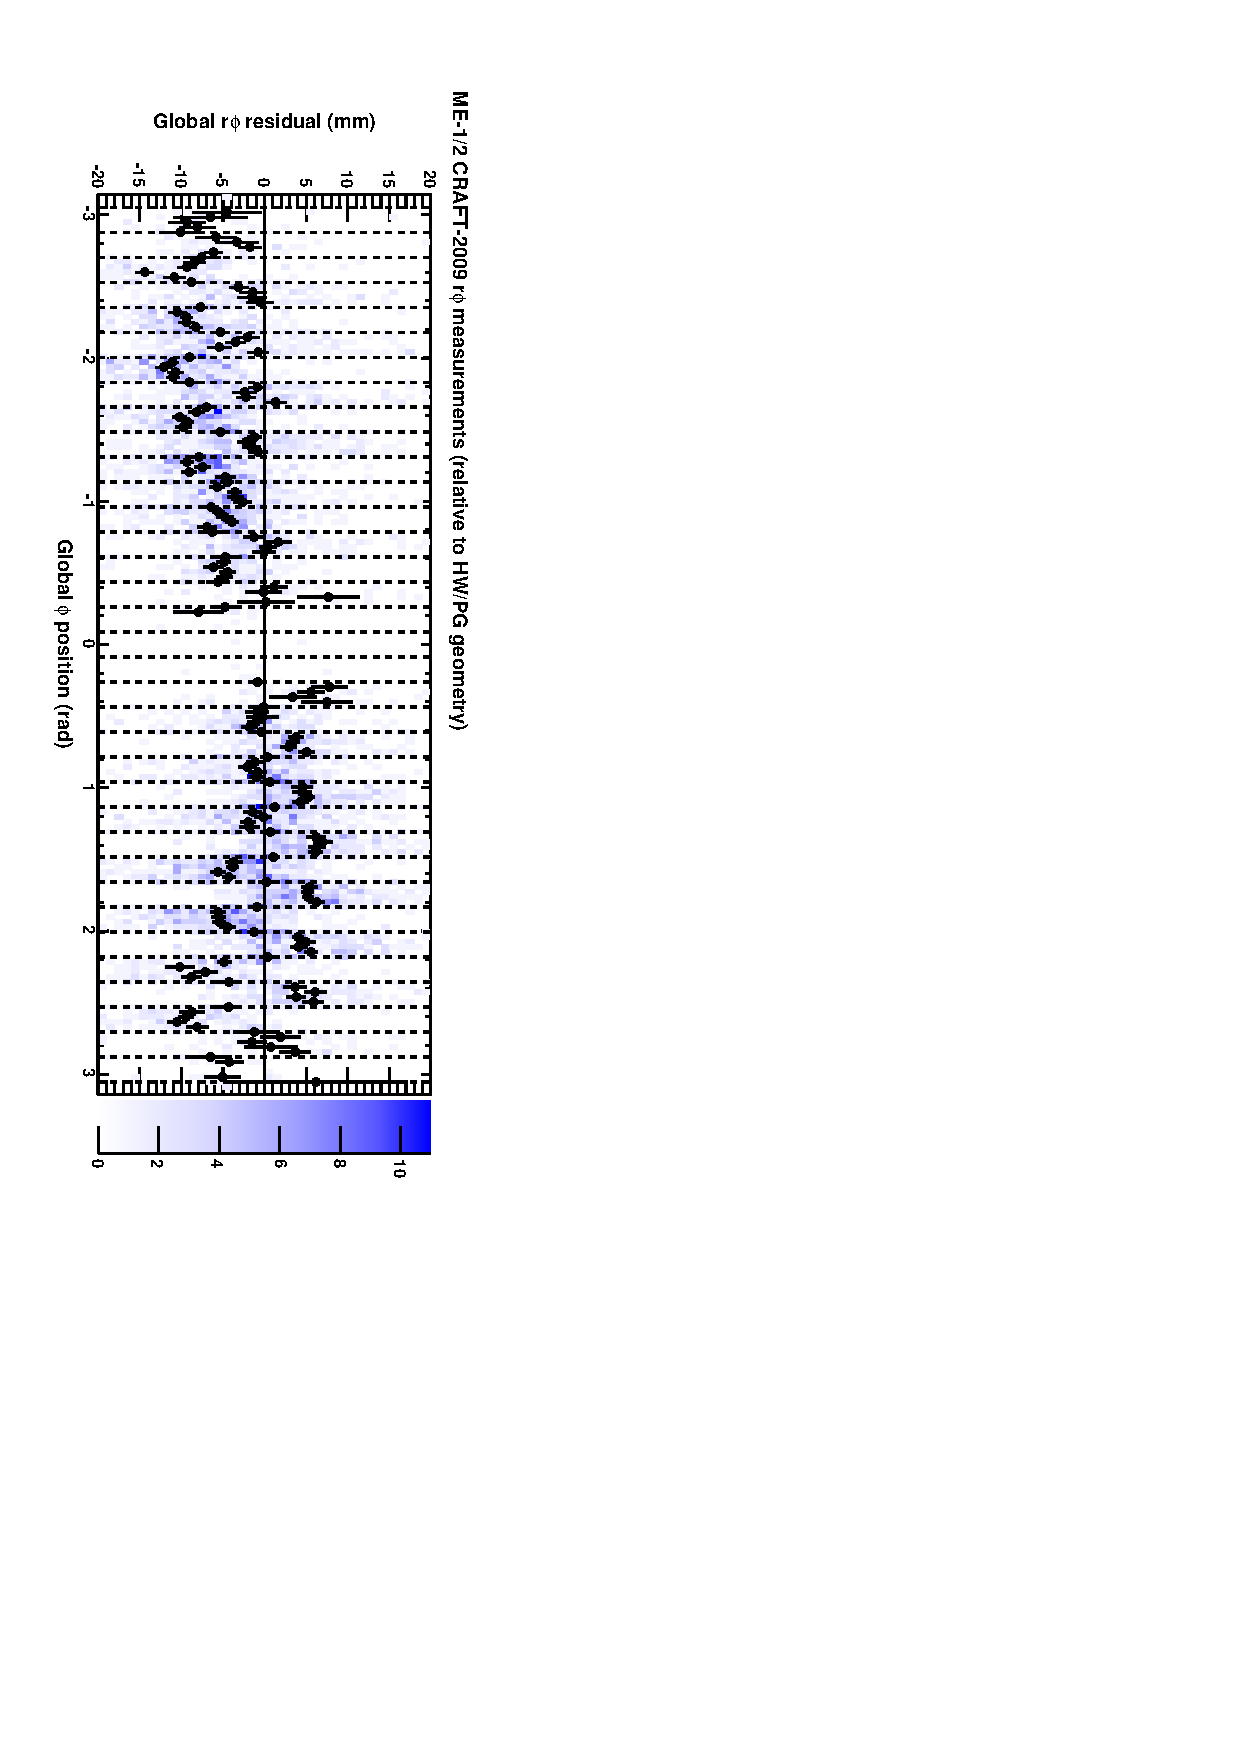
\includegraphics[height=\linewidth, angle=90]{alternation_2009_mem12_hwpg.pdf}
\end{frame}

\begin{frame}
\frametitle{The other projection}
\framesubtitle{Selected two neighboring chambers and plot vs.~$R$; nothing strange}

\vspace{0.2 cm}
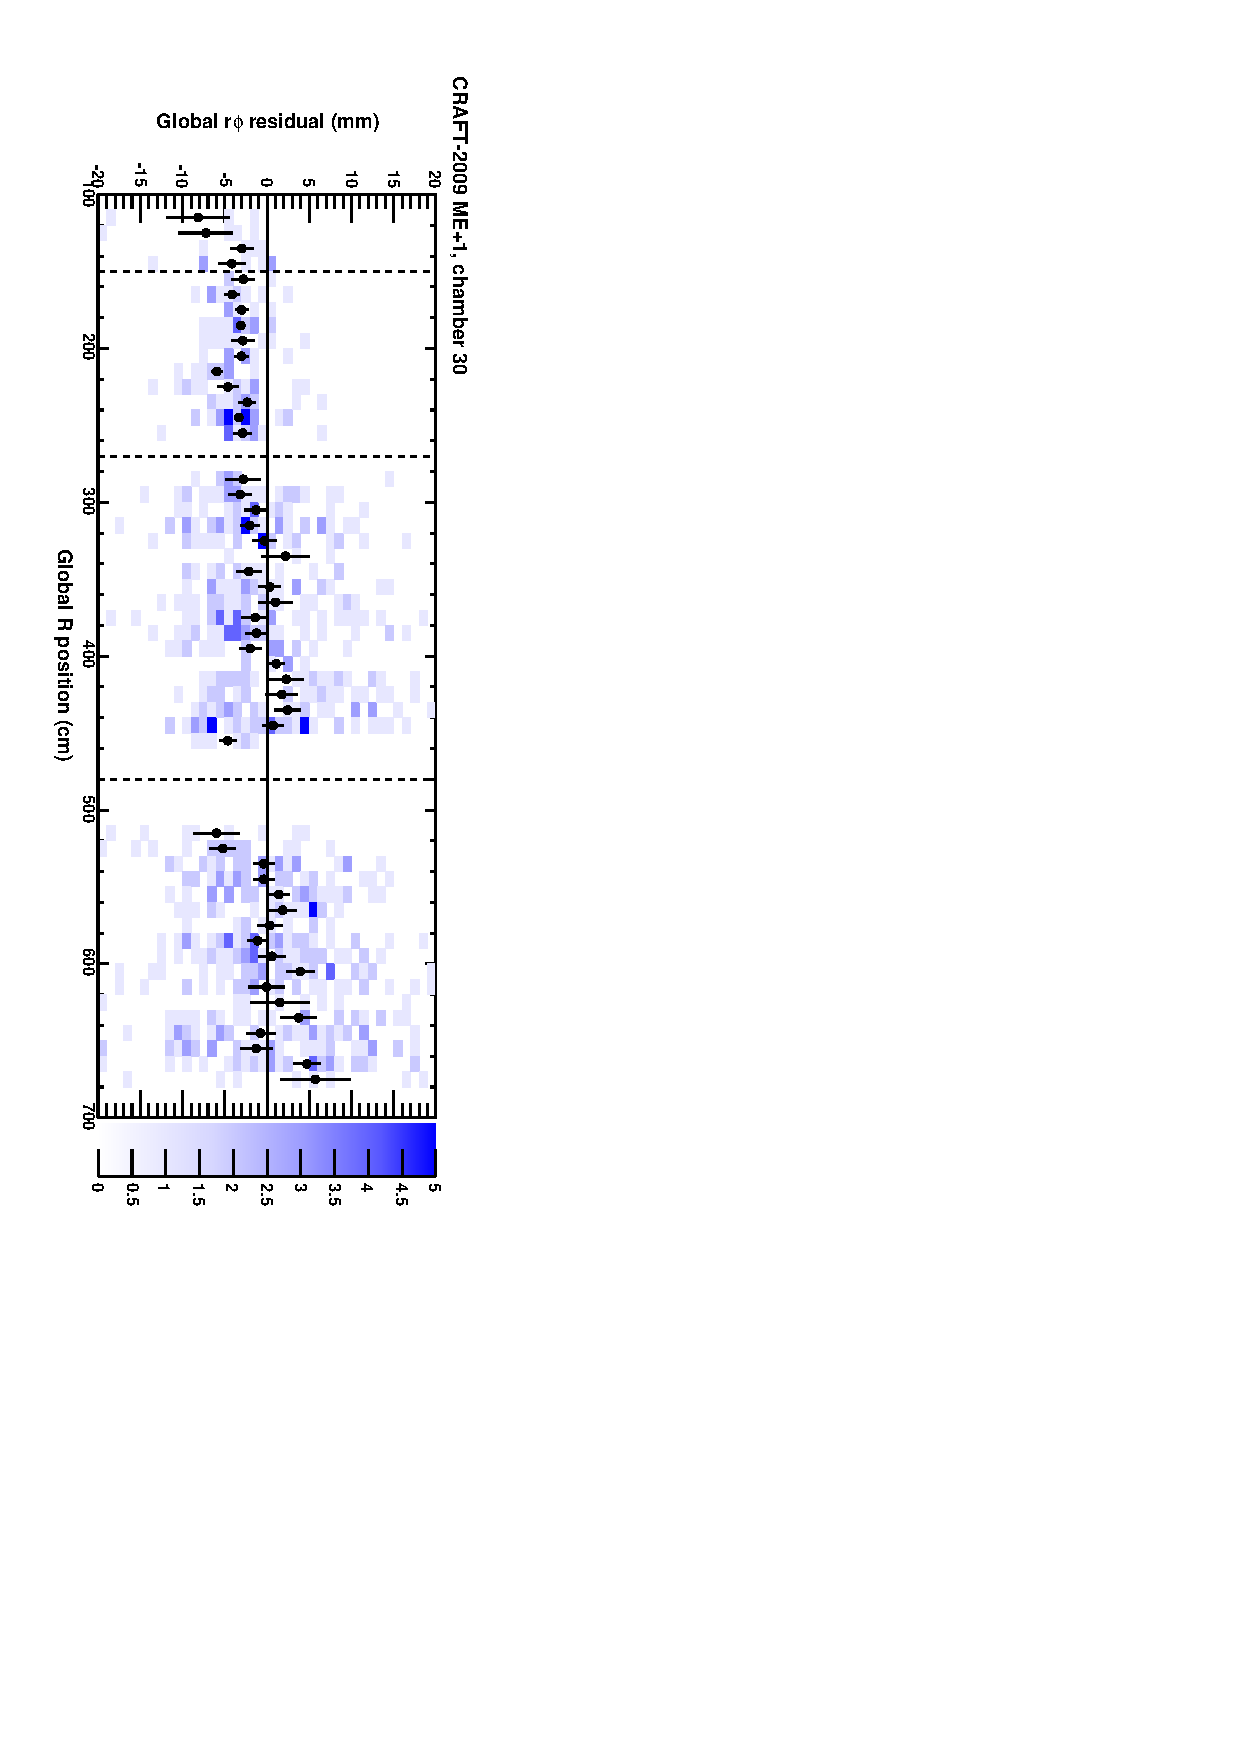
\includegraphics[height=\linewidth, angle=90]{alternation_2009-30.pdf}

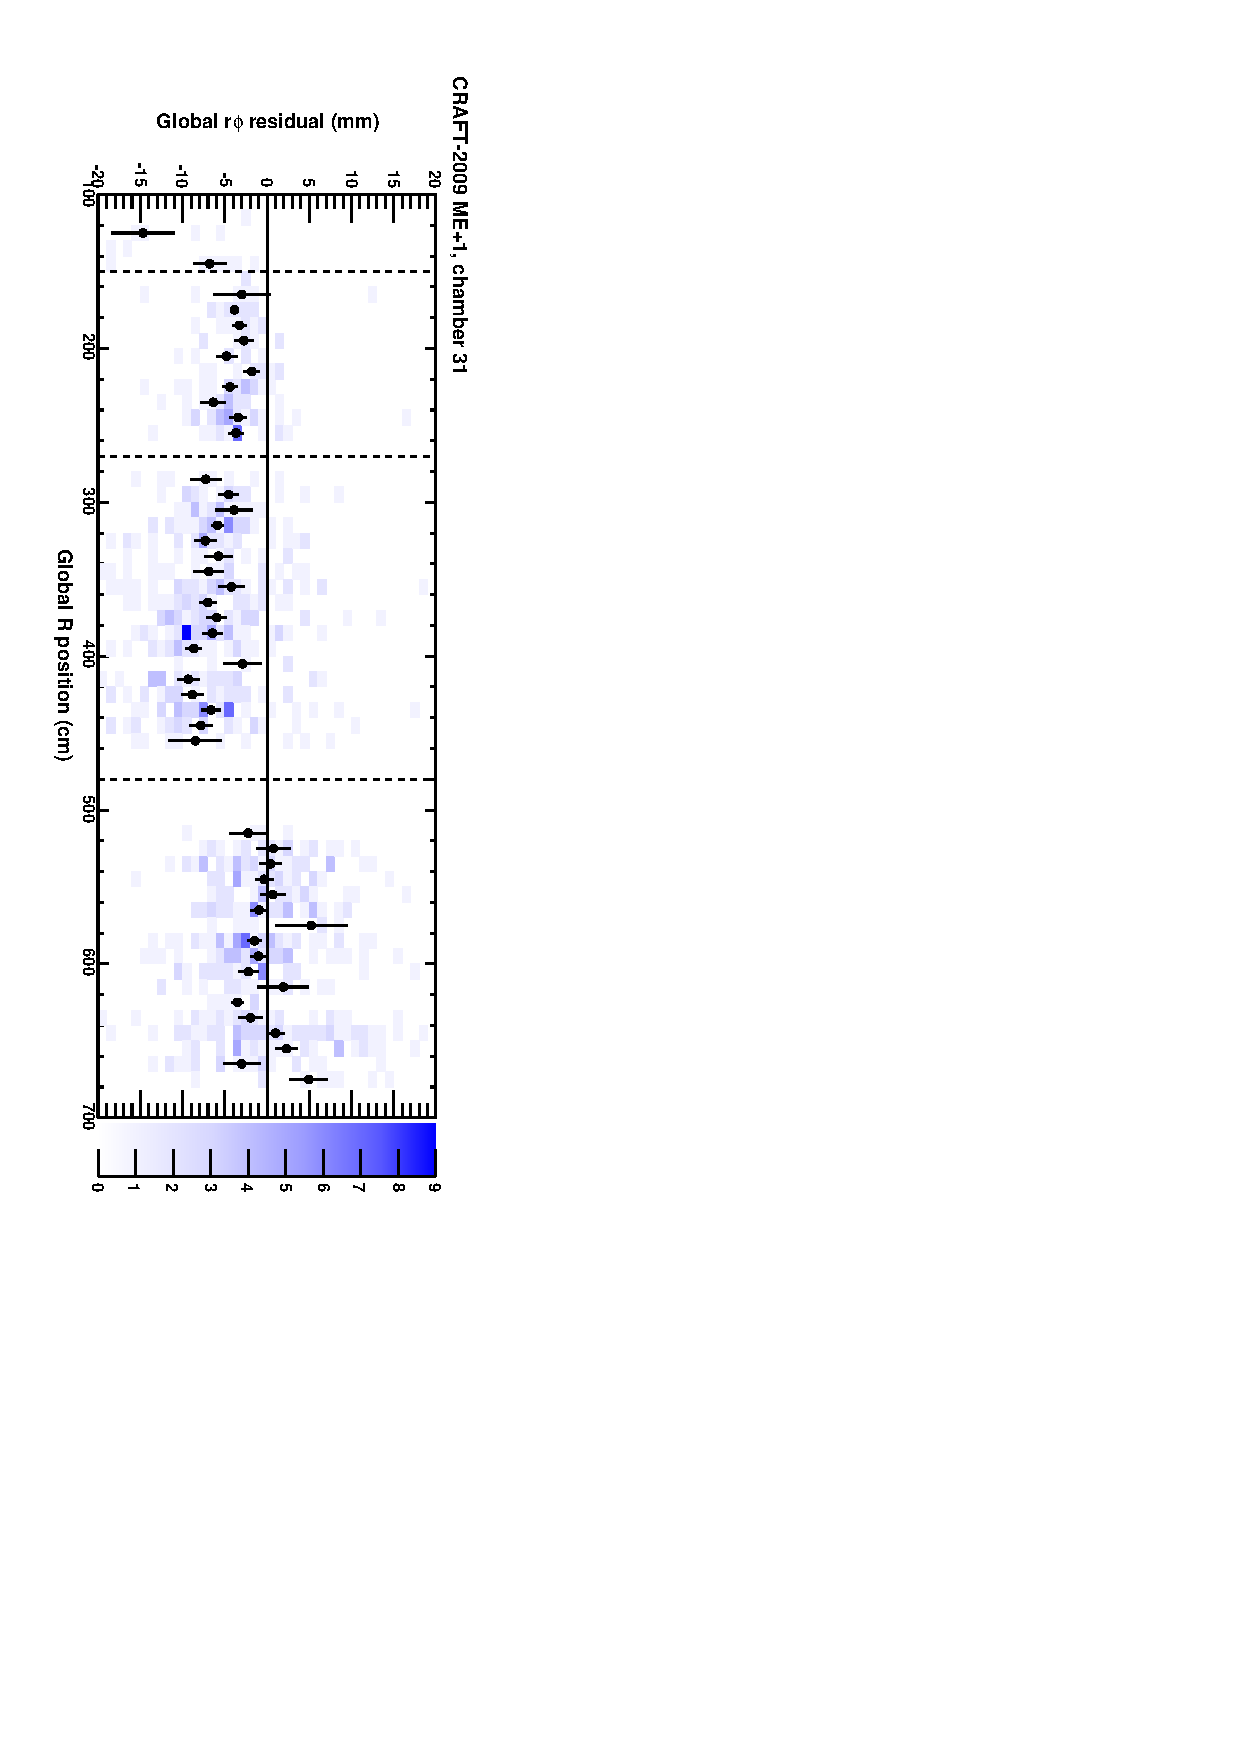
\includegraphics[height=\linewidth, angle=90]{alternation_2009-31.pdf}
\end{frame}

\begin{frame}
\frametitle{Summary of alteration pattern}

\begin{itemize}\setlength{\itemsep}{0.25 cm}
\item Only affects ME$\pm x$/2.  ME$\pm x$/1 look fine and ME$\pm$1/3
  has a pattern of its own
\item Complete set of $\Delta r\phi$ vs.~$\phi$ in backup at the end of this talk
\item Reconstruction bug?  Has something to do with local
  reconstruction or the local $\to$ global coordinate transformation\ldots
\begin{itemize}
\item alignment residuals constructed from CSCRecHit2Ds
\item same plotting code: only CMSSW version for tracks changed
  (CMSSW\_3\_1\_2, rather than 2\_2\_11)
\end{itemize}

\item Apart from this, we're in a position to do a high-quality disk alignment
\end{itemize}
\end{frame}

\begin{frame}
\frametitle{Alignment of ME$+$4/2?}
\framesubtitle{They exist and are not obviously misaligned; not clear if they alternate}

\vspace{0.2 cm}
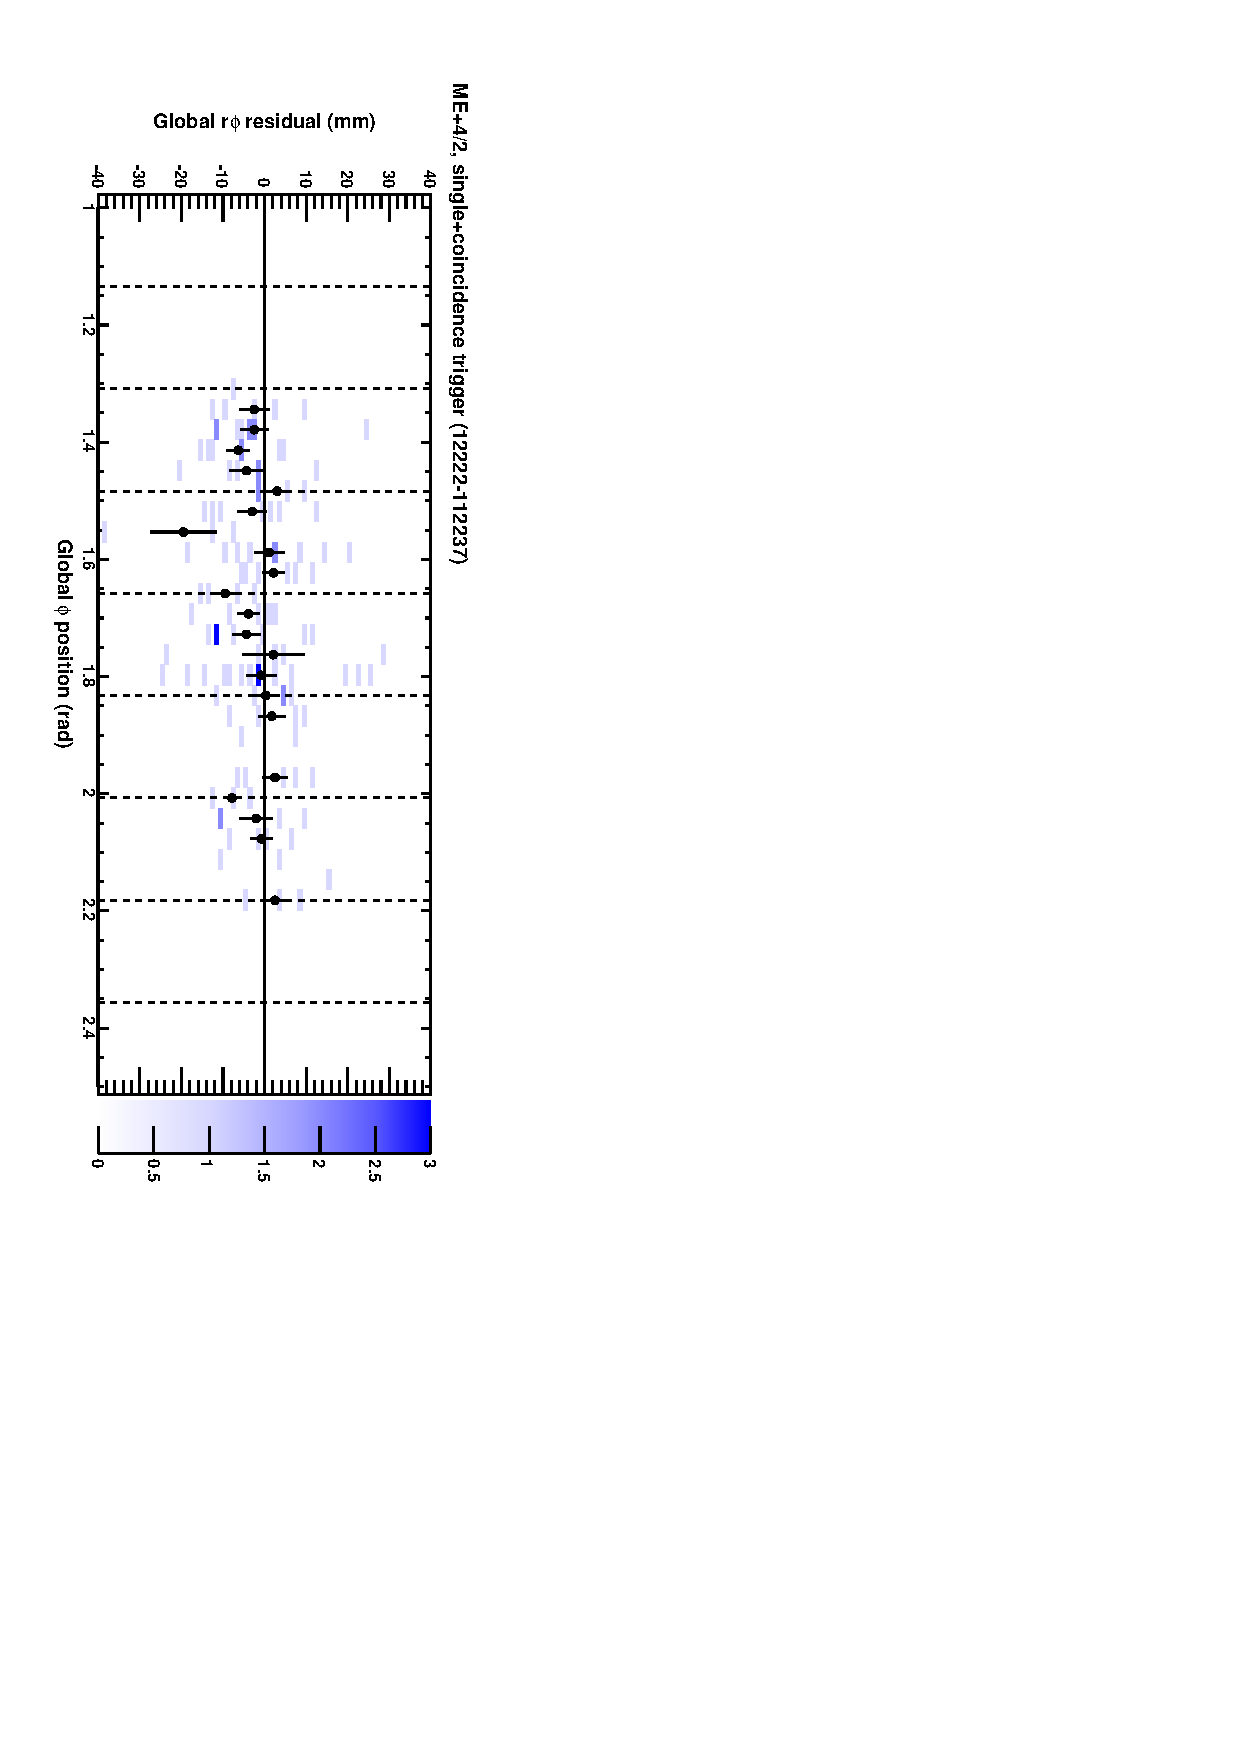
\includegraphics[height=\linewidth, angle=90]{mep42_singcoin.pdf}

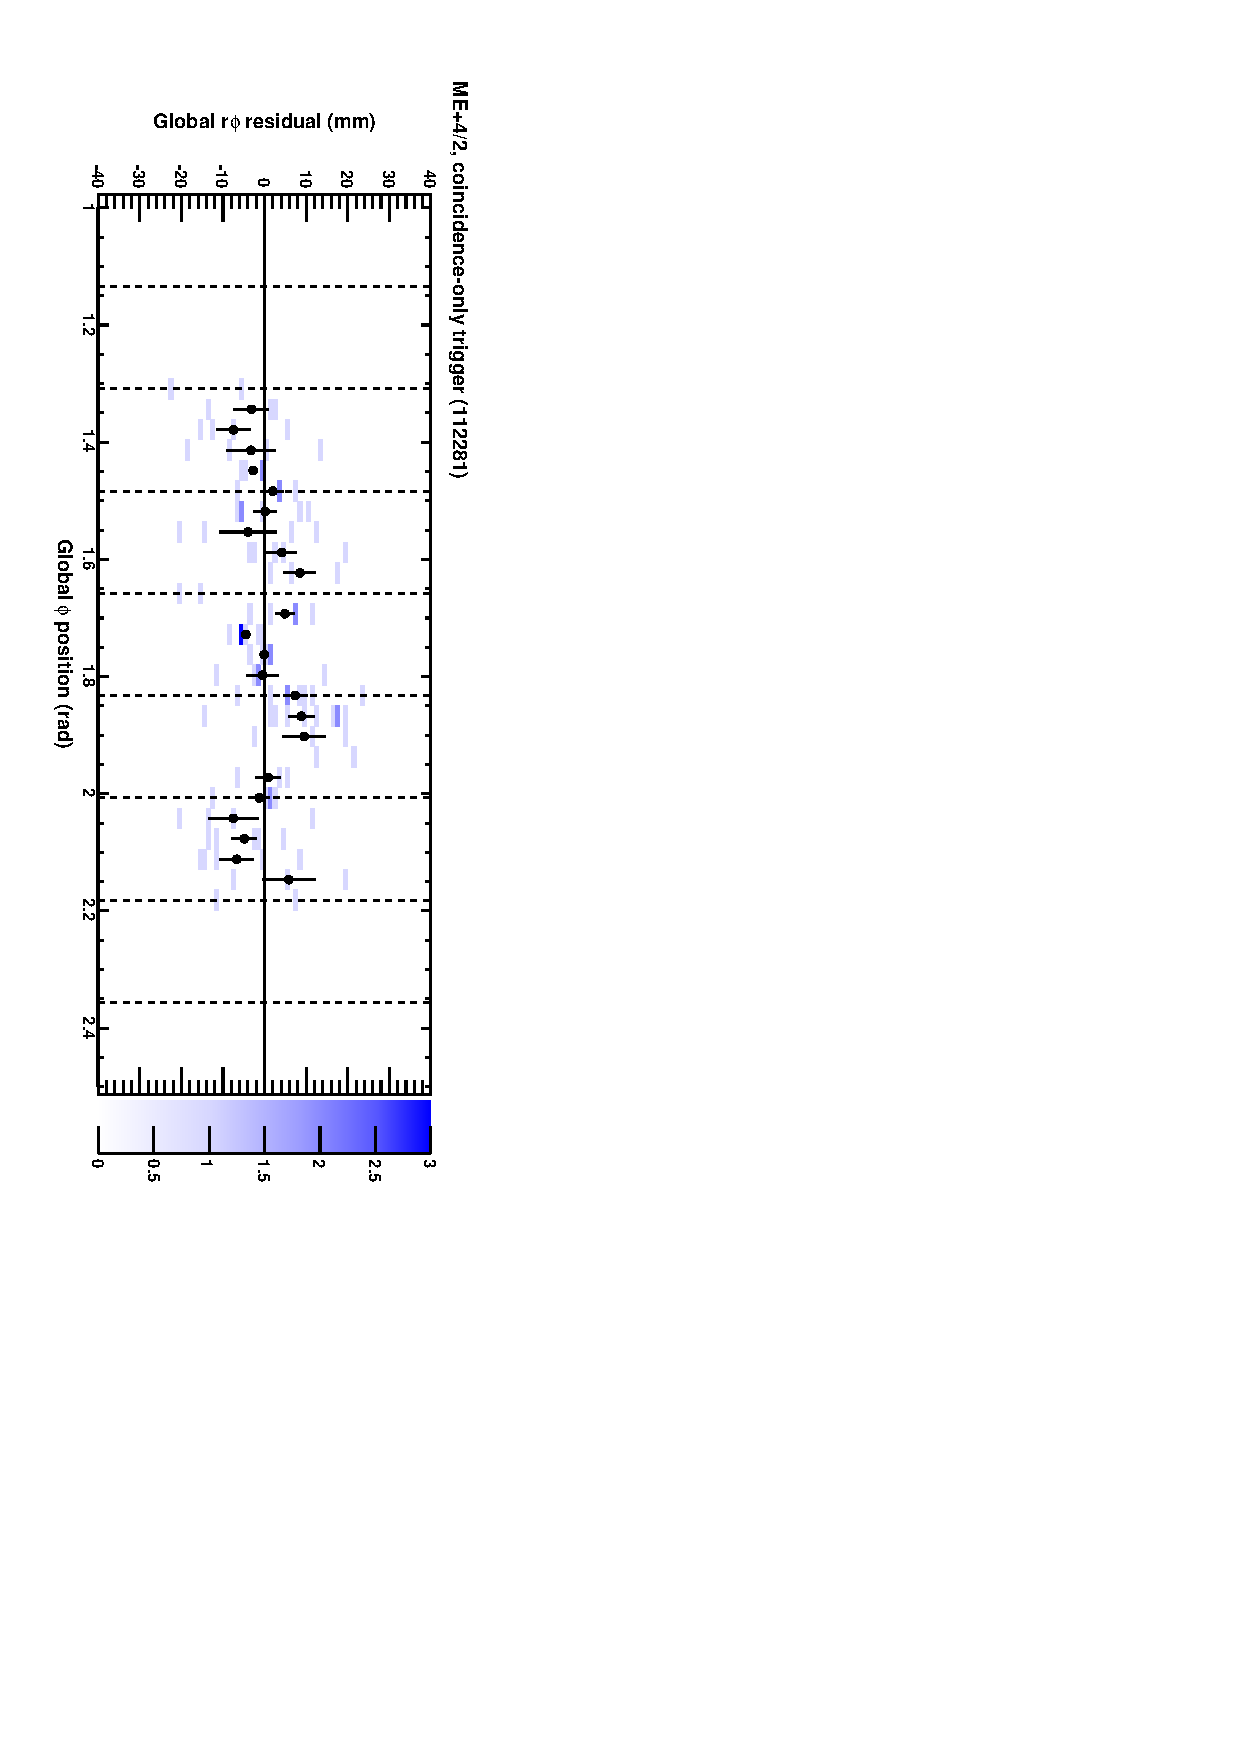
\includegraphics[height=\linewidth, angle=90]{mep42_coinonly.pdf}
\end{frame}

\begin{frame}
\frametitle{Work plans (conclusions)}

\textcolor{darkblue}{\large For the barrel}
\begin{itemize}
\item Minimum of changes, try to deliver aligned geometry quickly
\item Possible changes:
\begin{itemize}
\item allow TID/TEC in track fits; if difference is small, include
  them
\item align parts of wheels~$\pm$2
\item fix $\phi_x$ to their photogrammetry values (5~DOF alignment)
\end{itemize}
\item Check compatibility of the three $\vec{B} = 3.8$~T periods
\end{itemize}

\vfill
\textcolor{darkblue}{\large For the endcap}
\begin{itemize}
\item Find and fix the alternation bug!  Could be in geometry, local
  reconstruction, track reconstruction
\item Align disks by hand in an interactive analysis (fit to
  $\mbox{const} + \sin\phi + \cos\phi$ curve)
\item Run automated procedure to align chamber $x$, $\phi_y$, and
  $\phi_z$ (small chamber corrections after large disk correction)
\end{itemize}
\label{numpages}
\end{frame}

%% \section*{First section}
%% \begin{frame}
%% \begin{center}
%% \Huge \textcolor{blue}{First section}
%% \end{center}
%% \end{frame}

\begin{frame}
\vspace{1 cm}
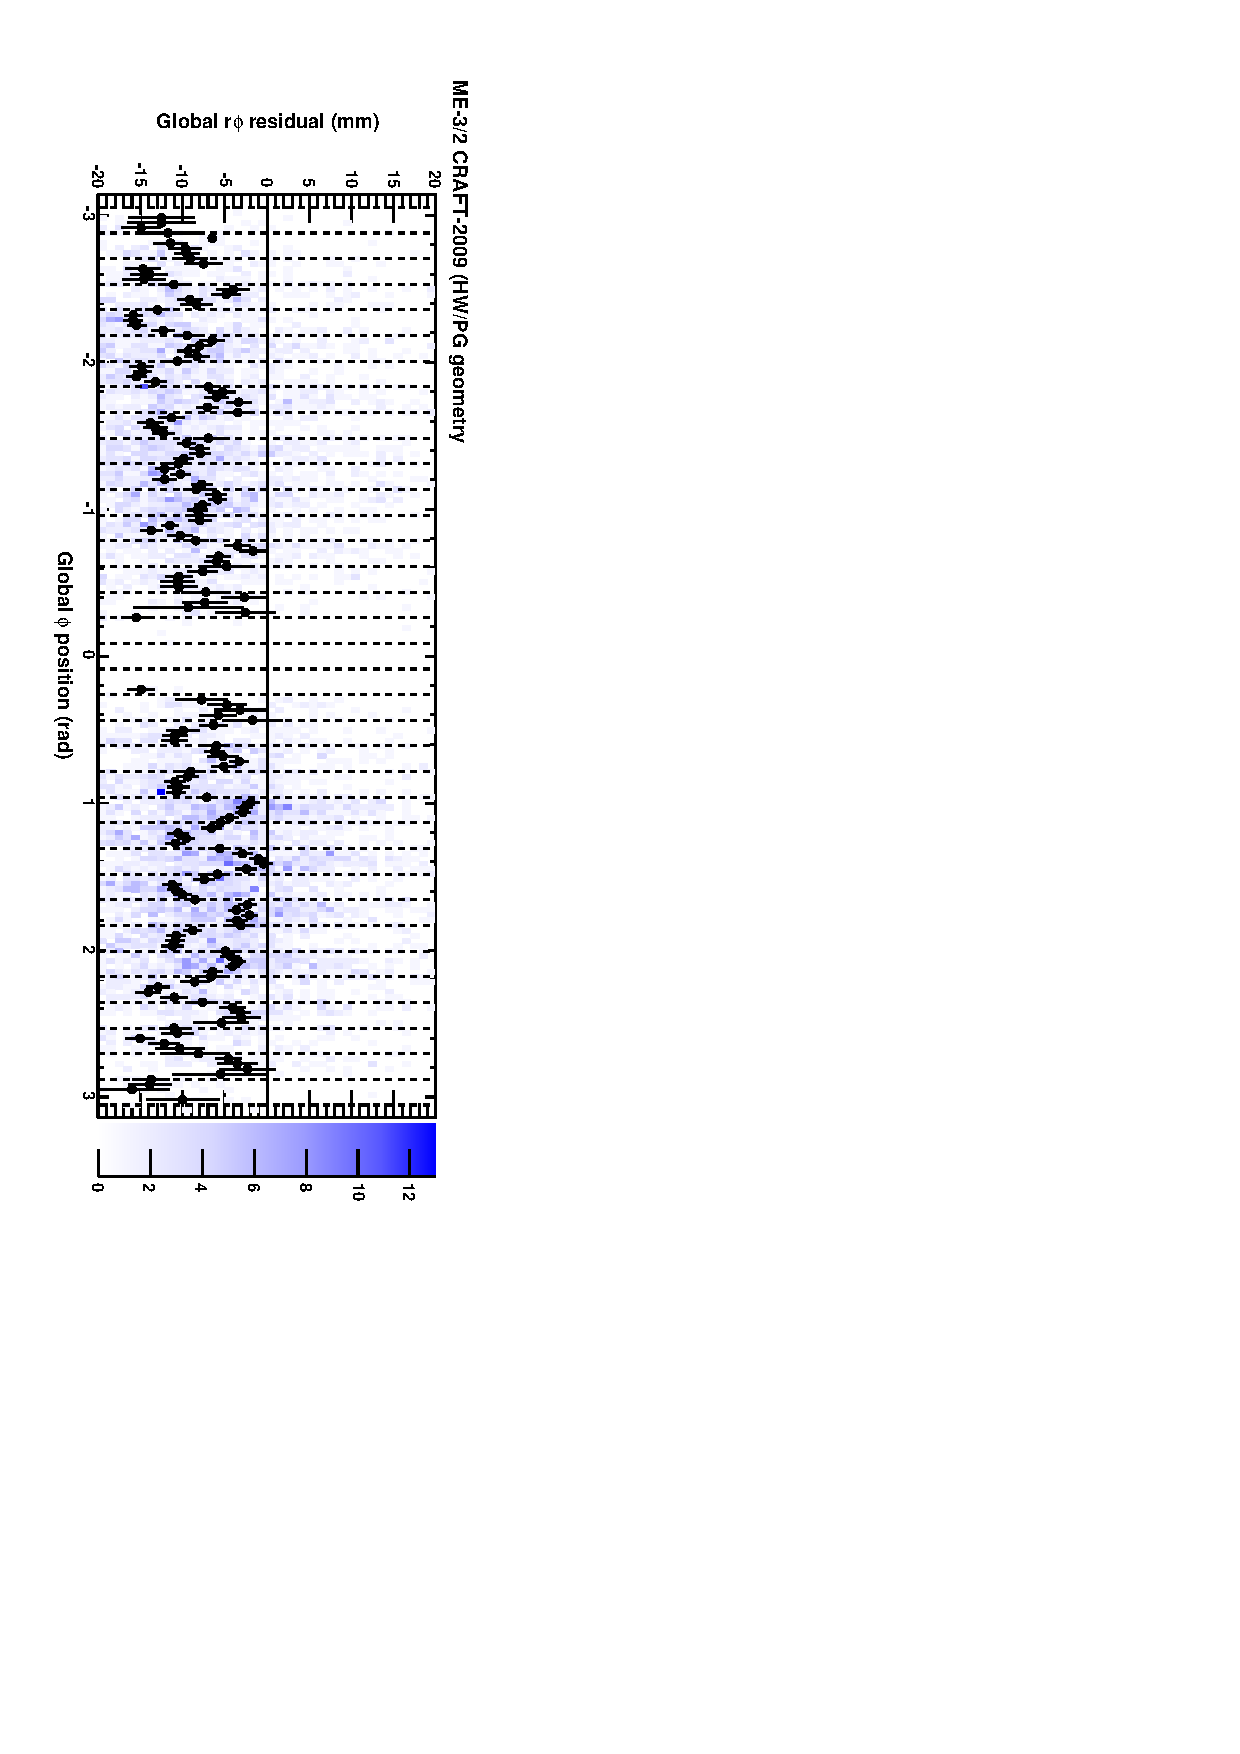
\includegraphics[height=\linewidth, angle=90]{series01.pdf}

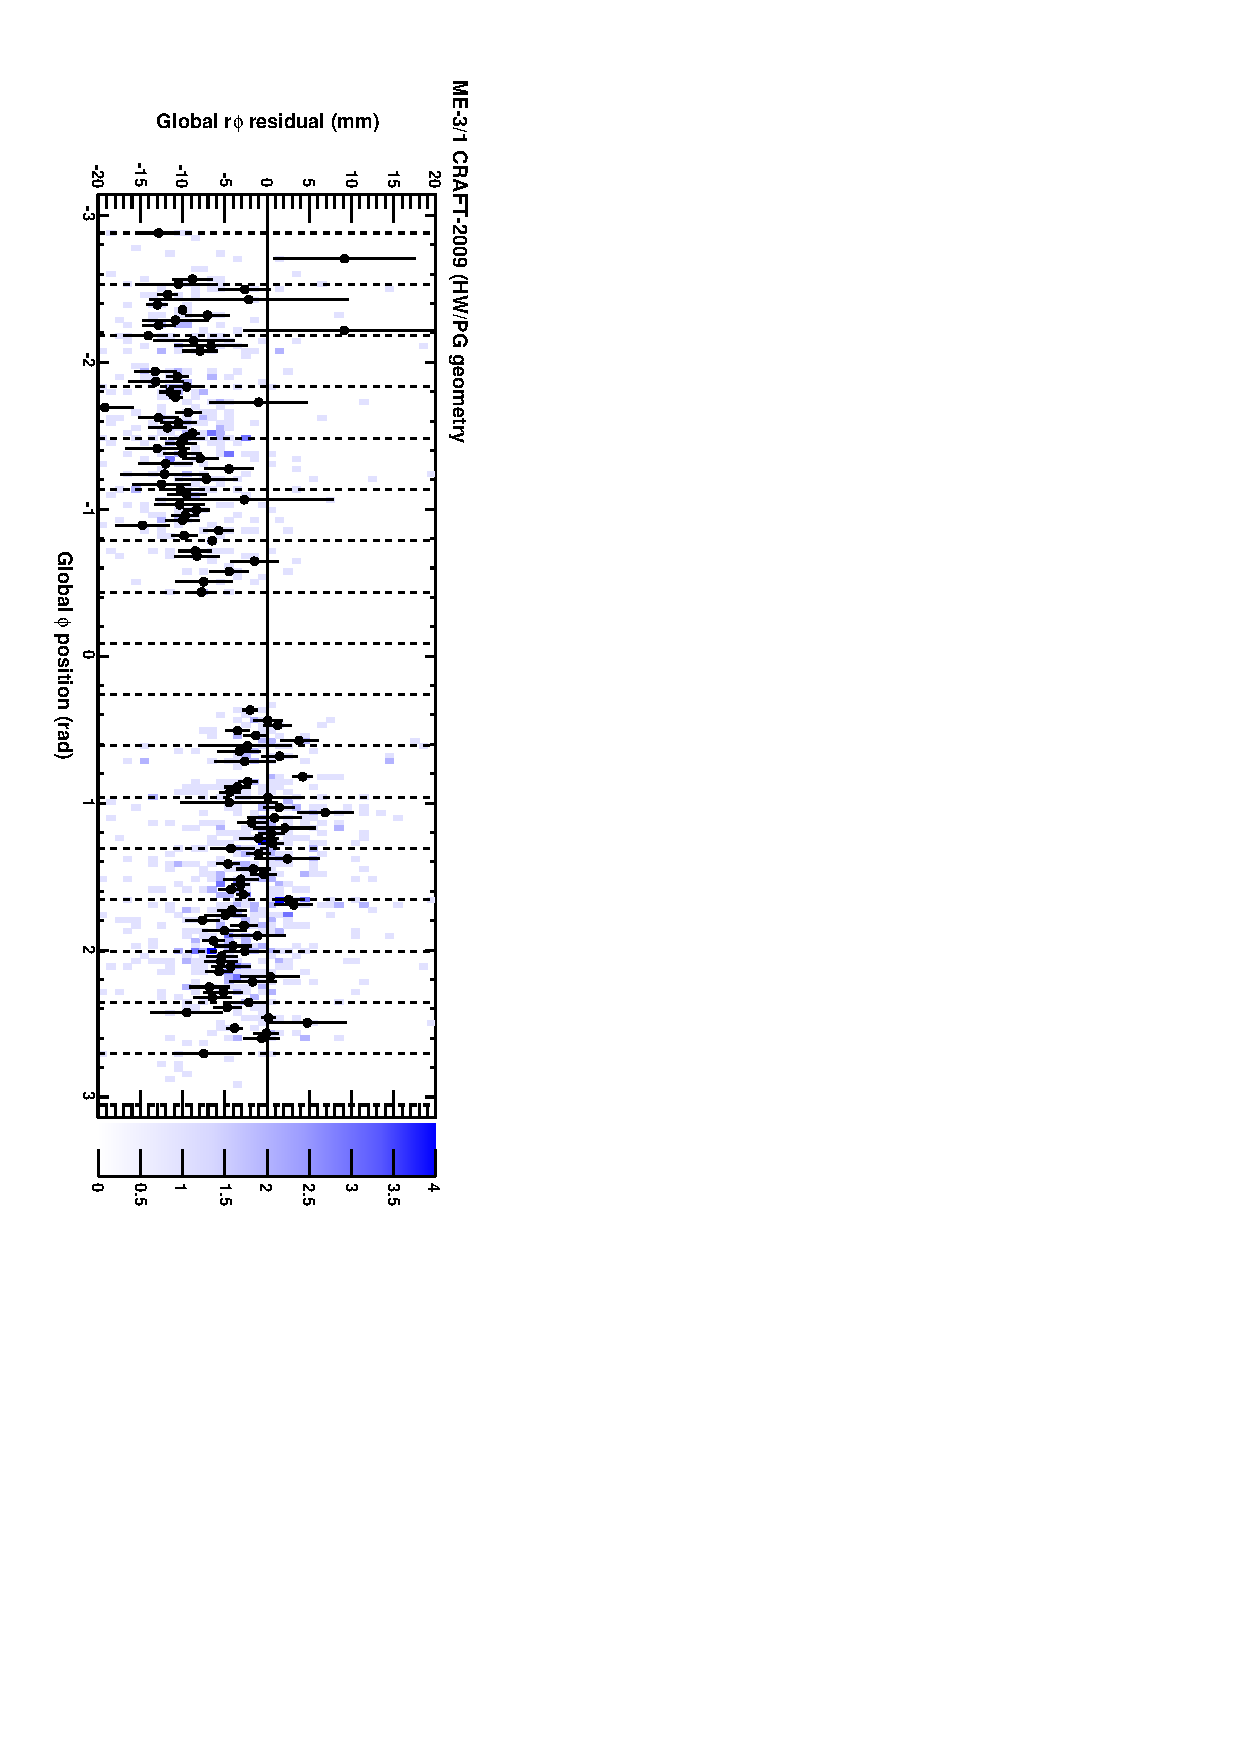
\includegraphics[height=\linewidth, angle=90]{series02.pdf}
\end{frame}

\begin{frame}
\vspace{1 cm}
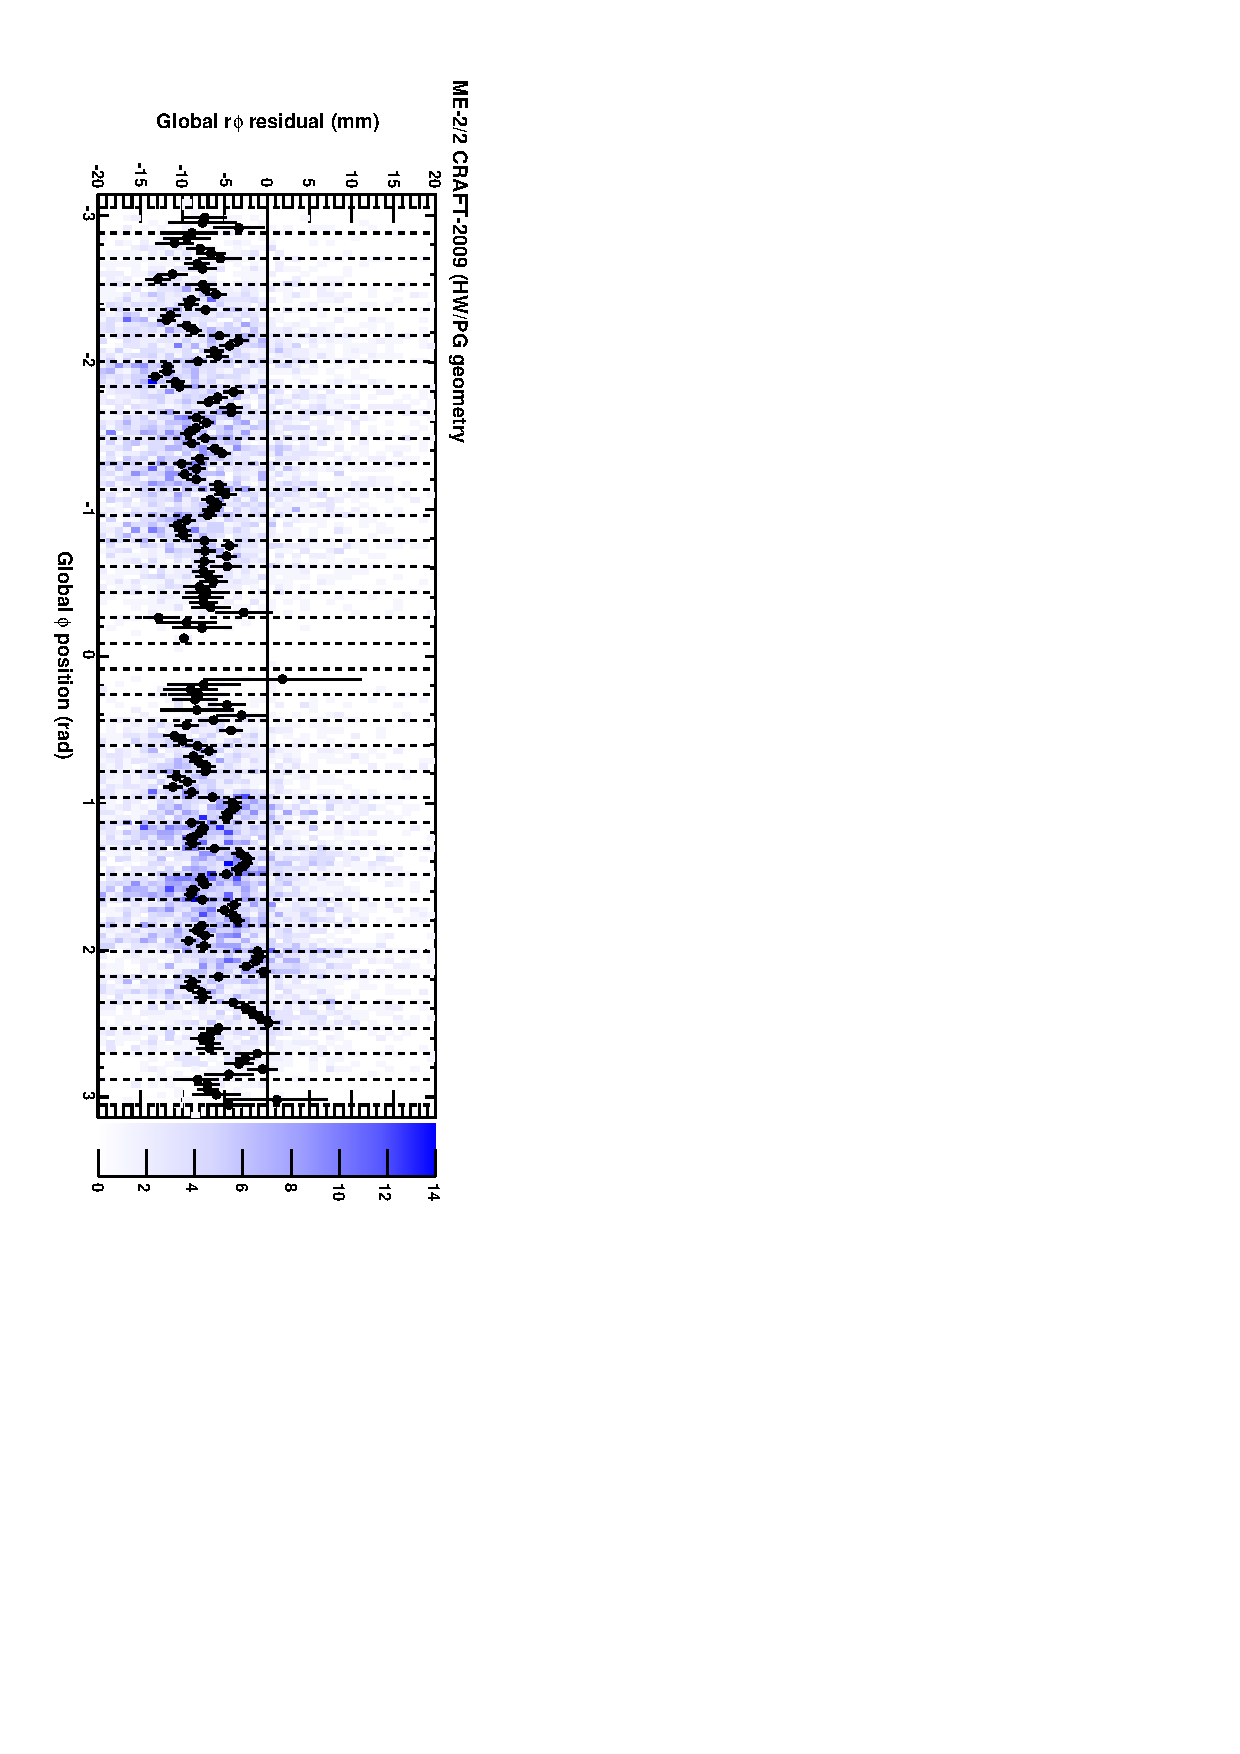
\includegraphics[height=\linewidth, angle=90]{series03.pdf}

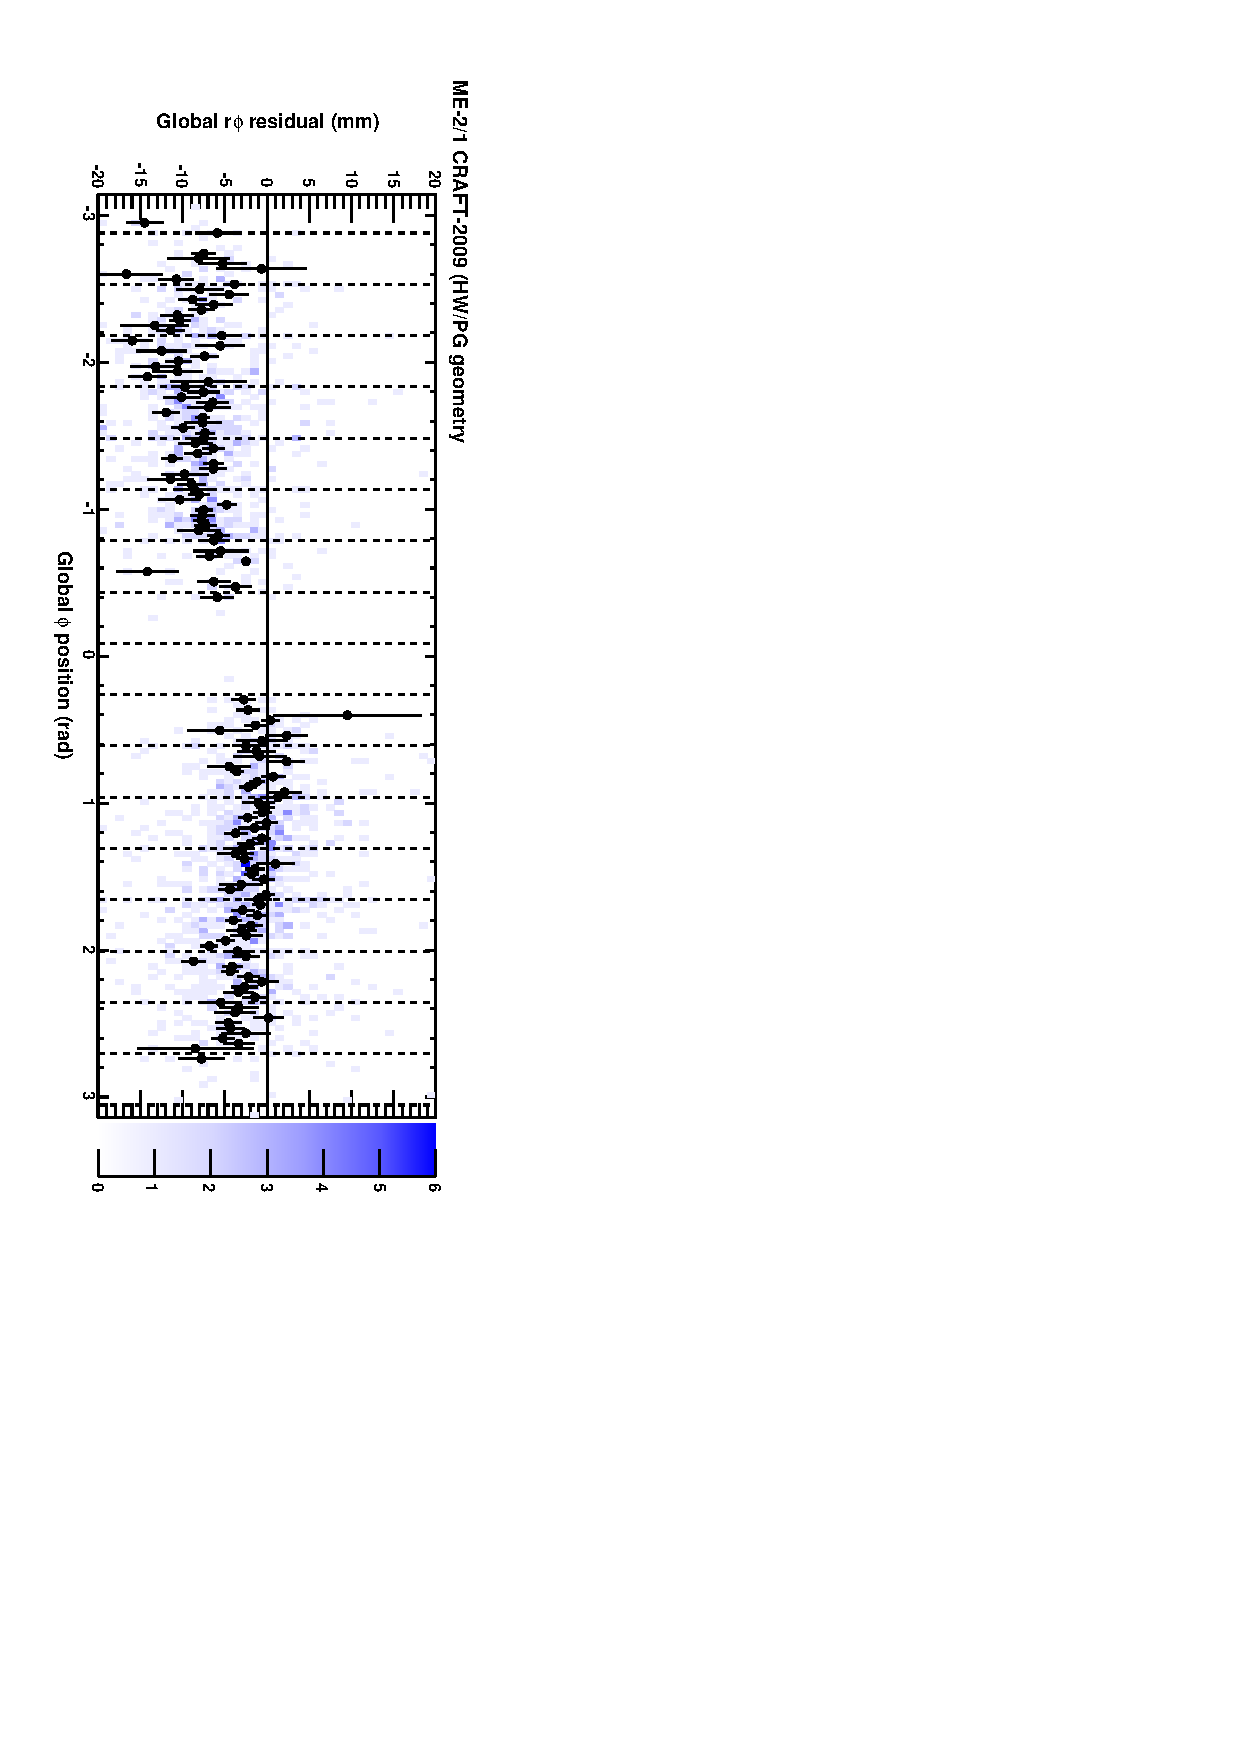
\includegraphics[height=\linewidth, angle=90]{series04.pdf}
\end{frame}

\begin{frame}
\vspace{0.5\baselineskip}
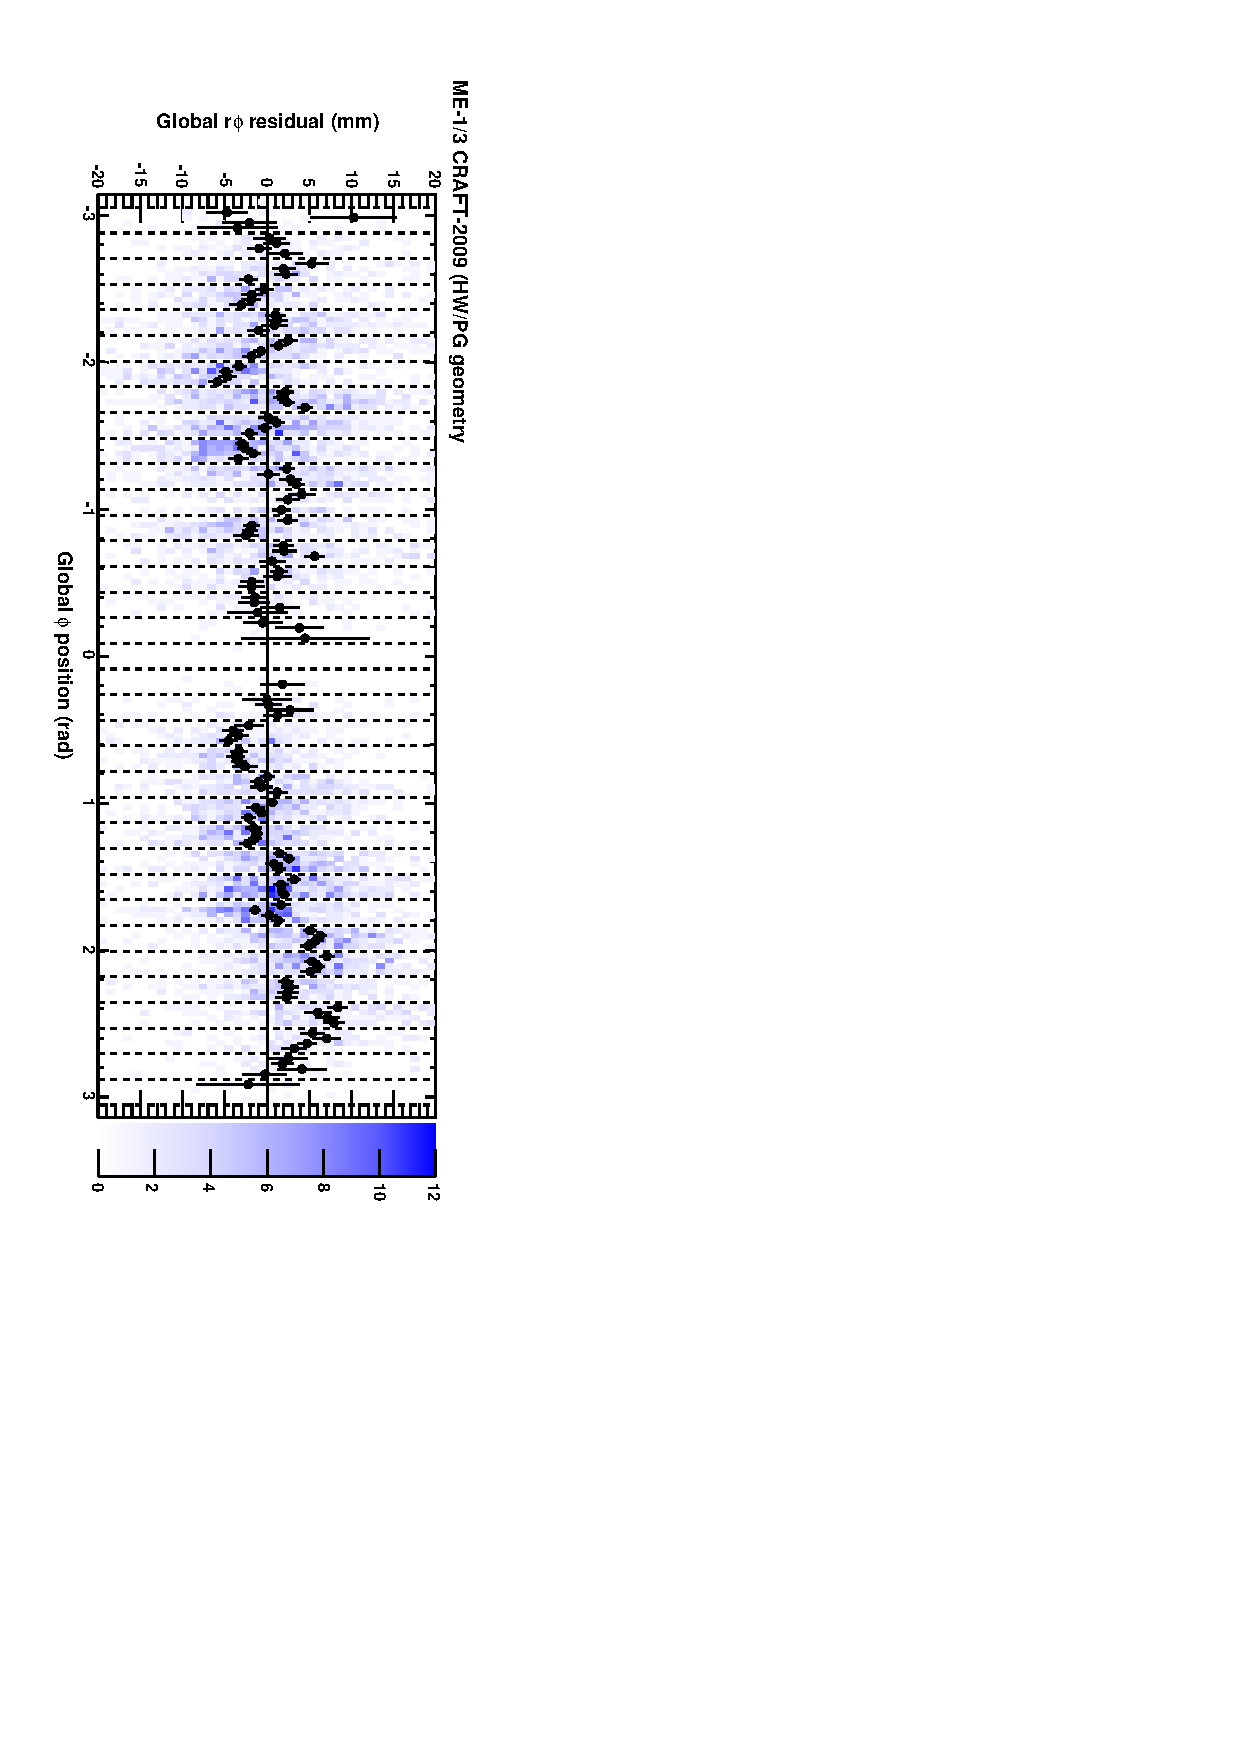
\includegraphics[height=0.75\linewidth, angle=90]{series05.pdf}

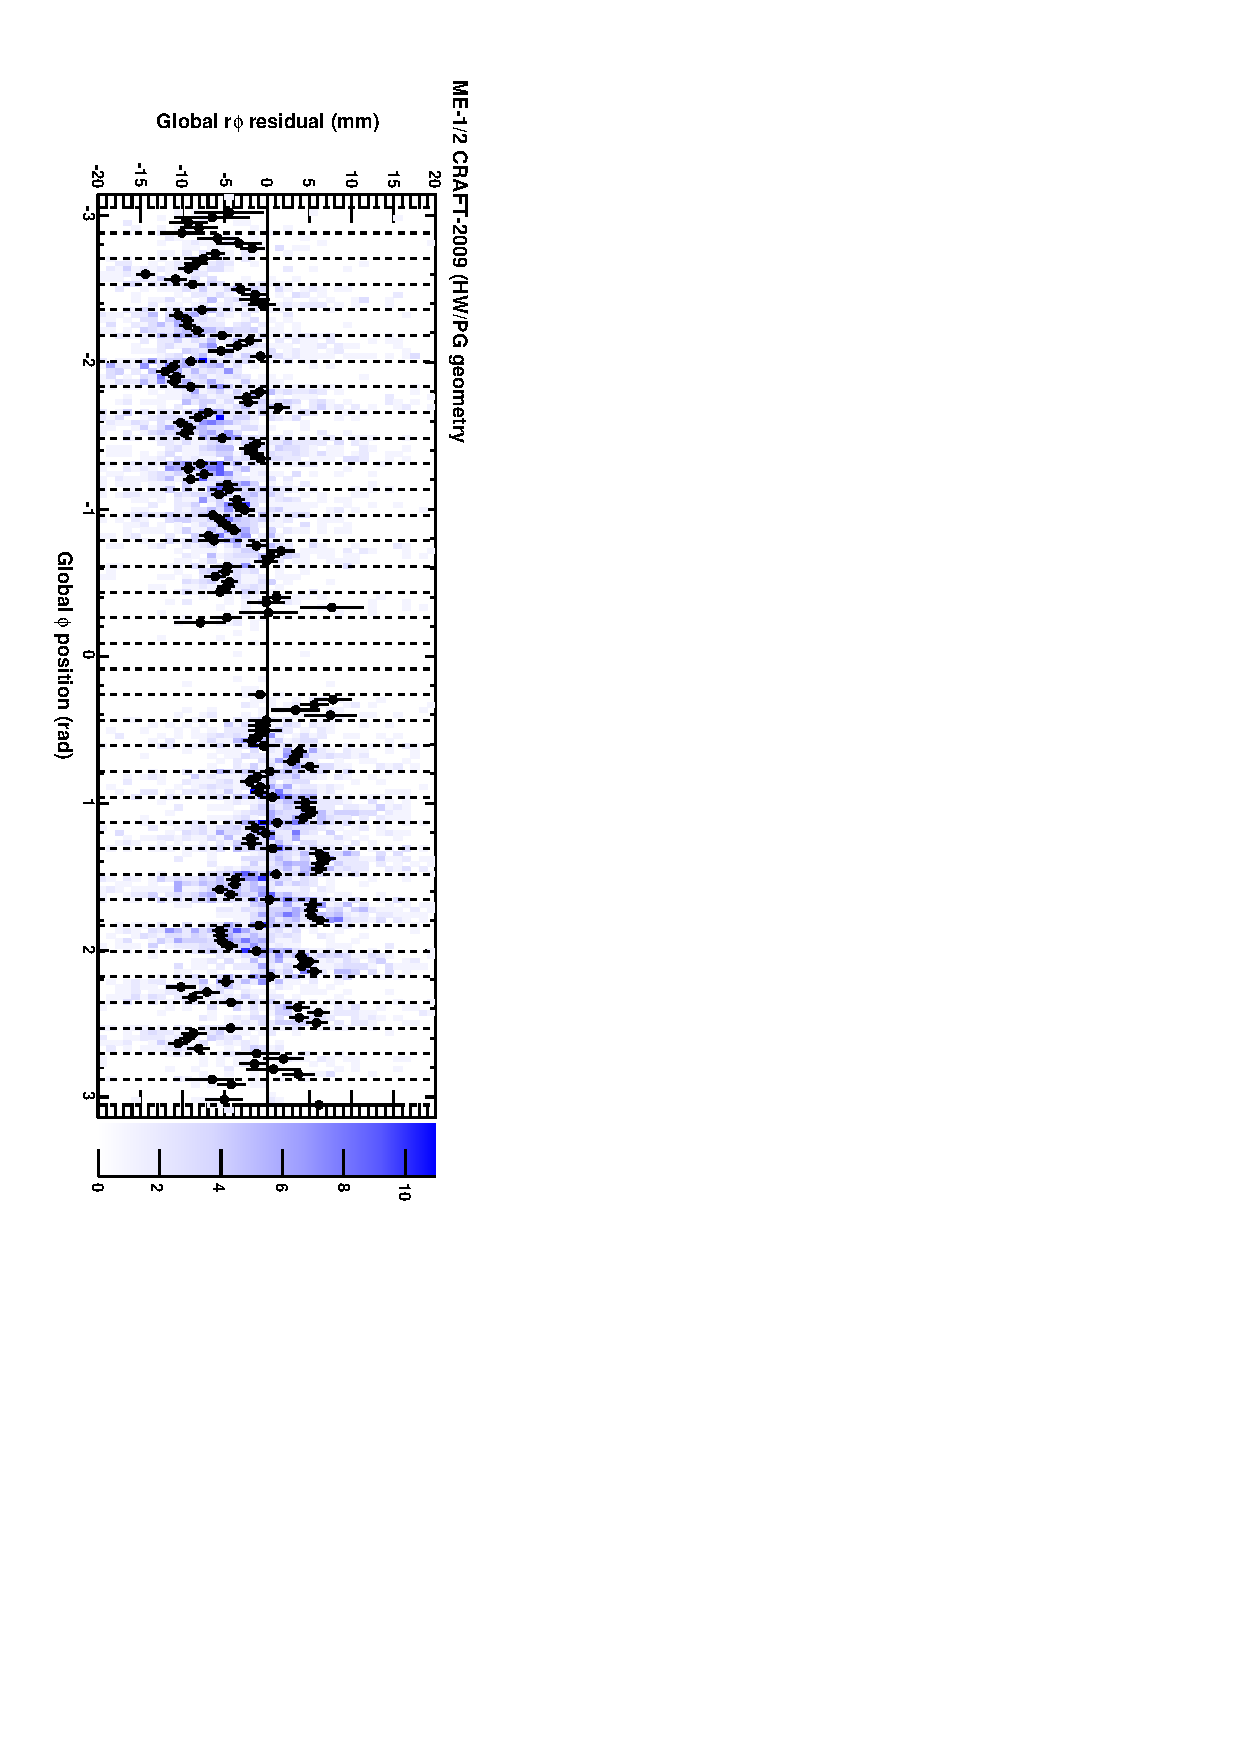
\includegraphics[height=0.75\linewidth, angle=90]{series06.pdf}

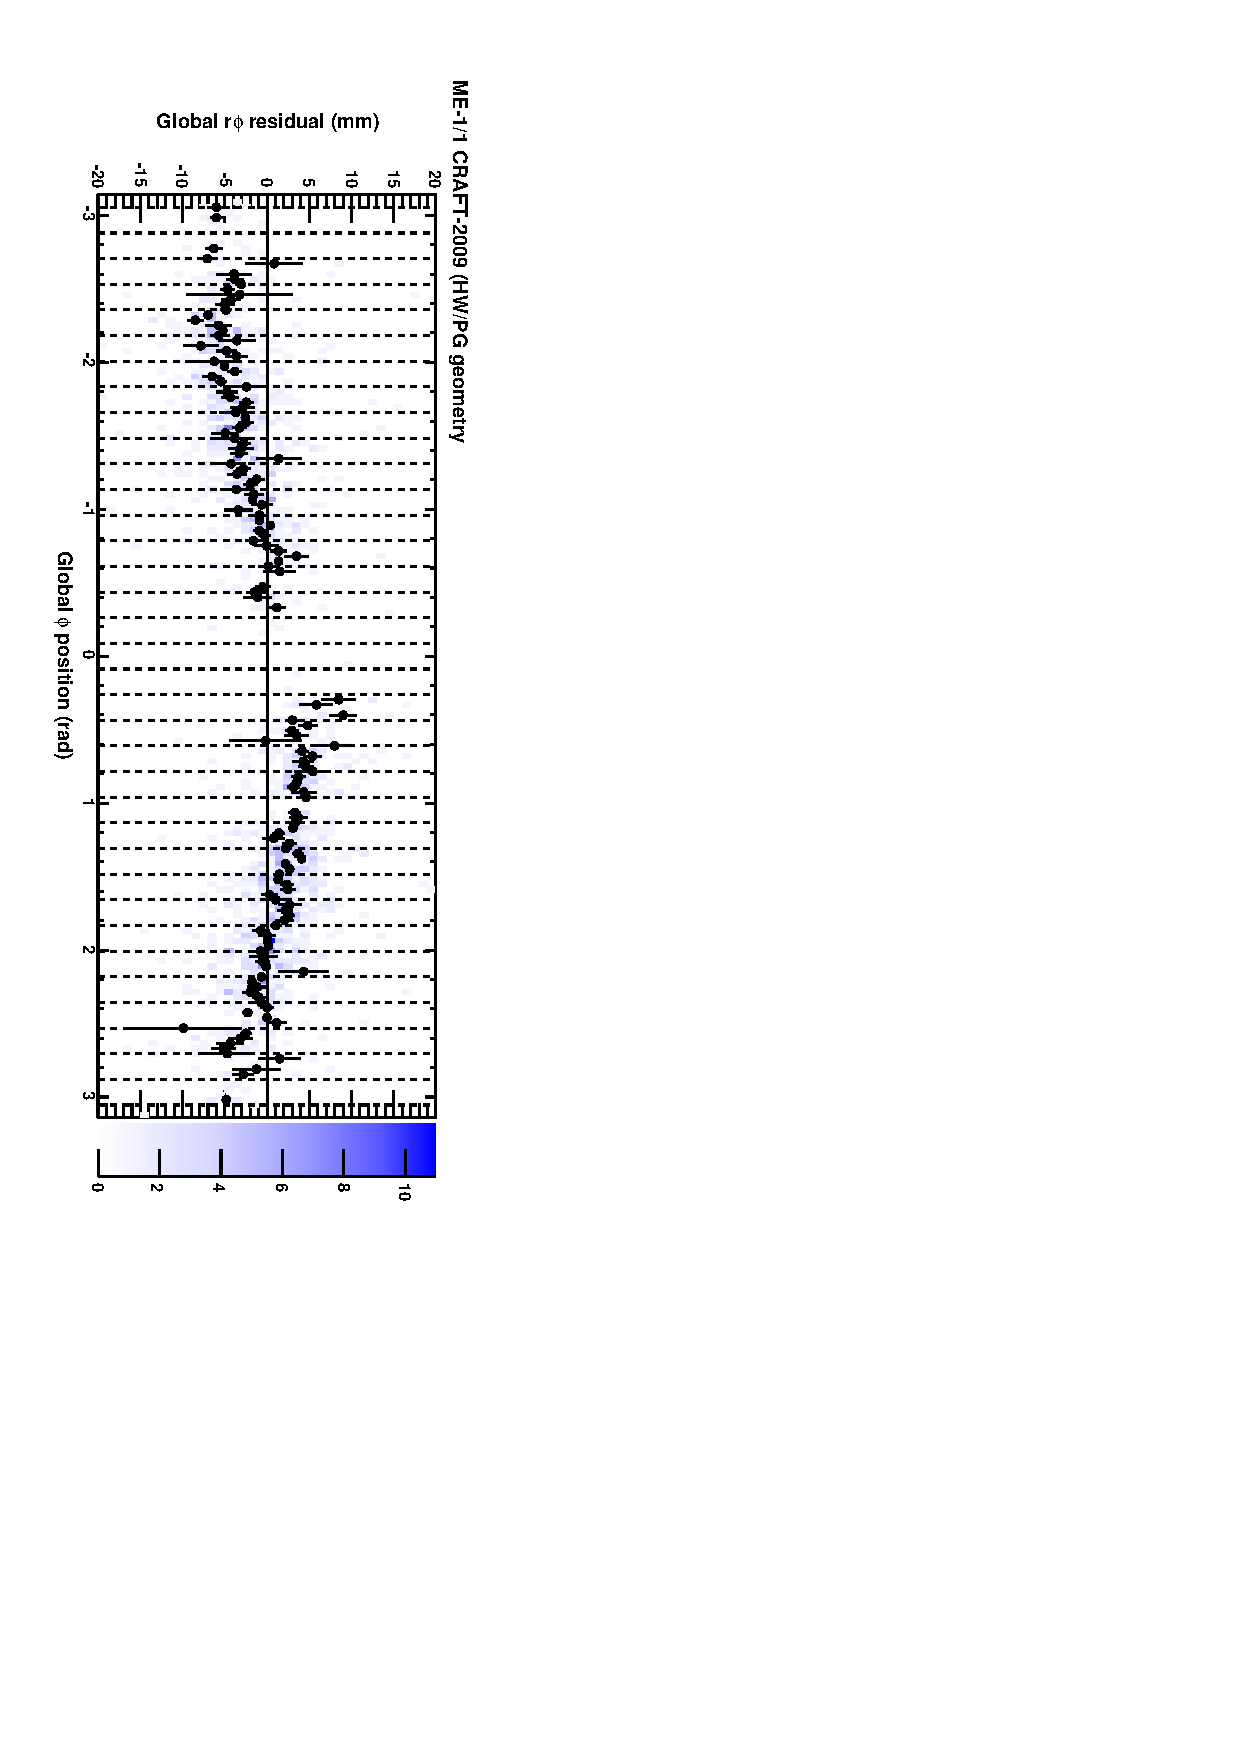
\includegraphics[height=0.75\linewidth, angle=90]{series07.pdf}
\end{frame}

\begin{frame}
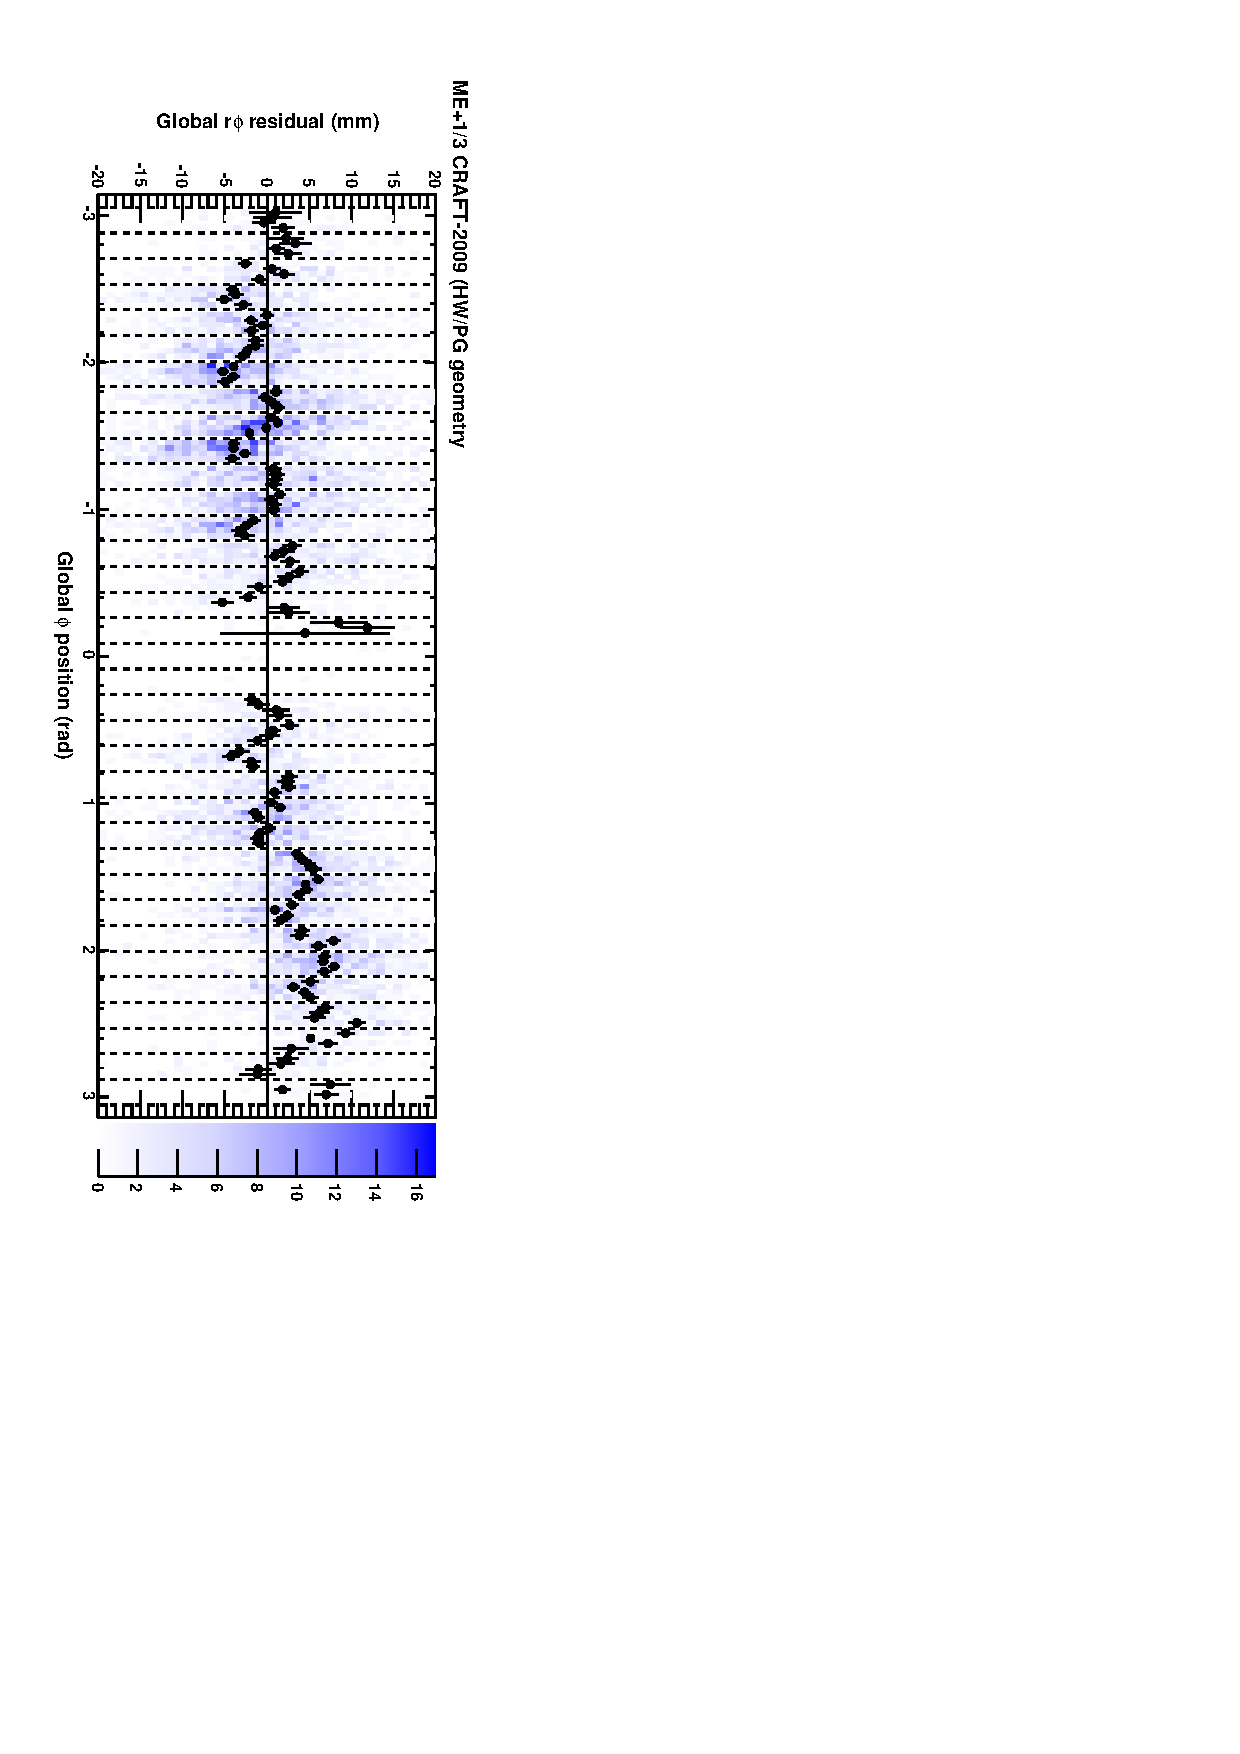
\includegraphics[height=0.75\linewidth, angle=90]{series10.pdf}

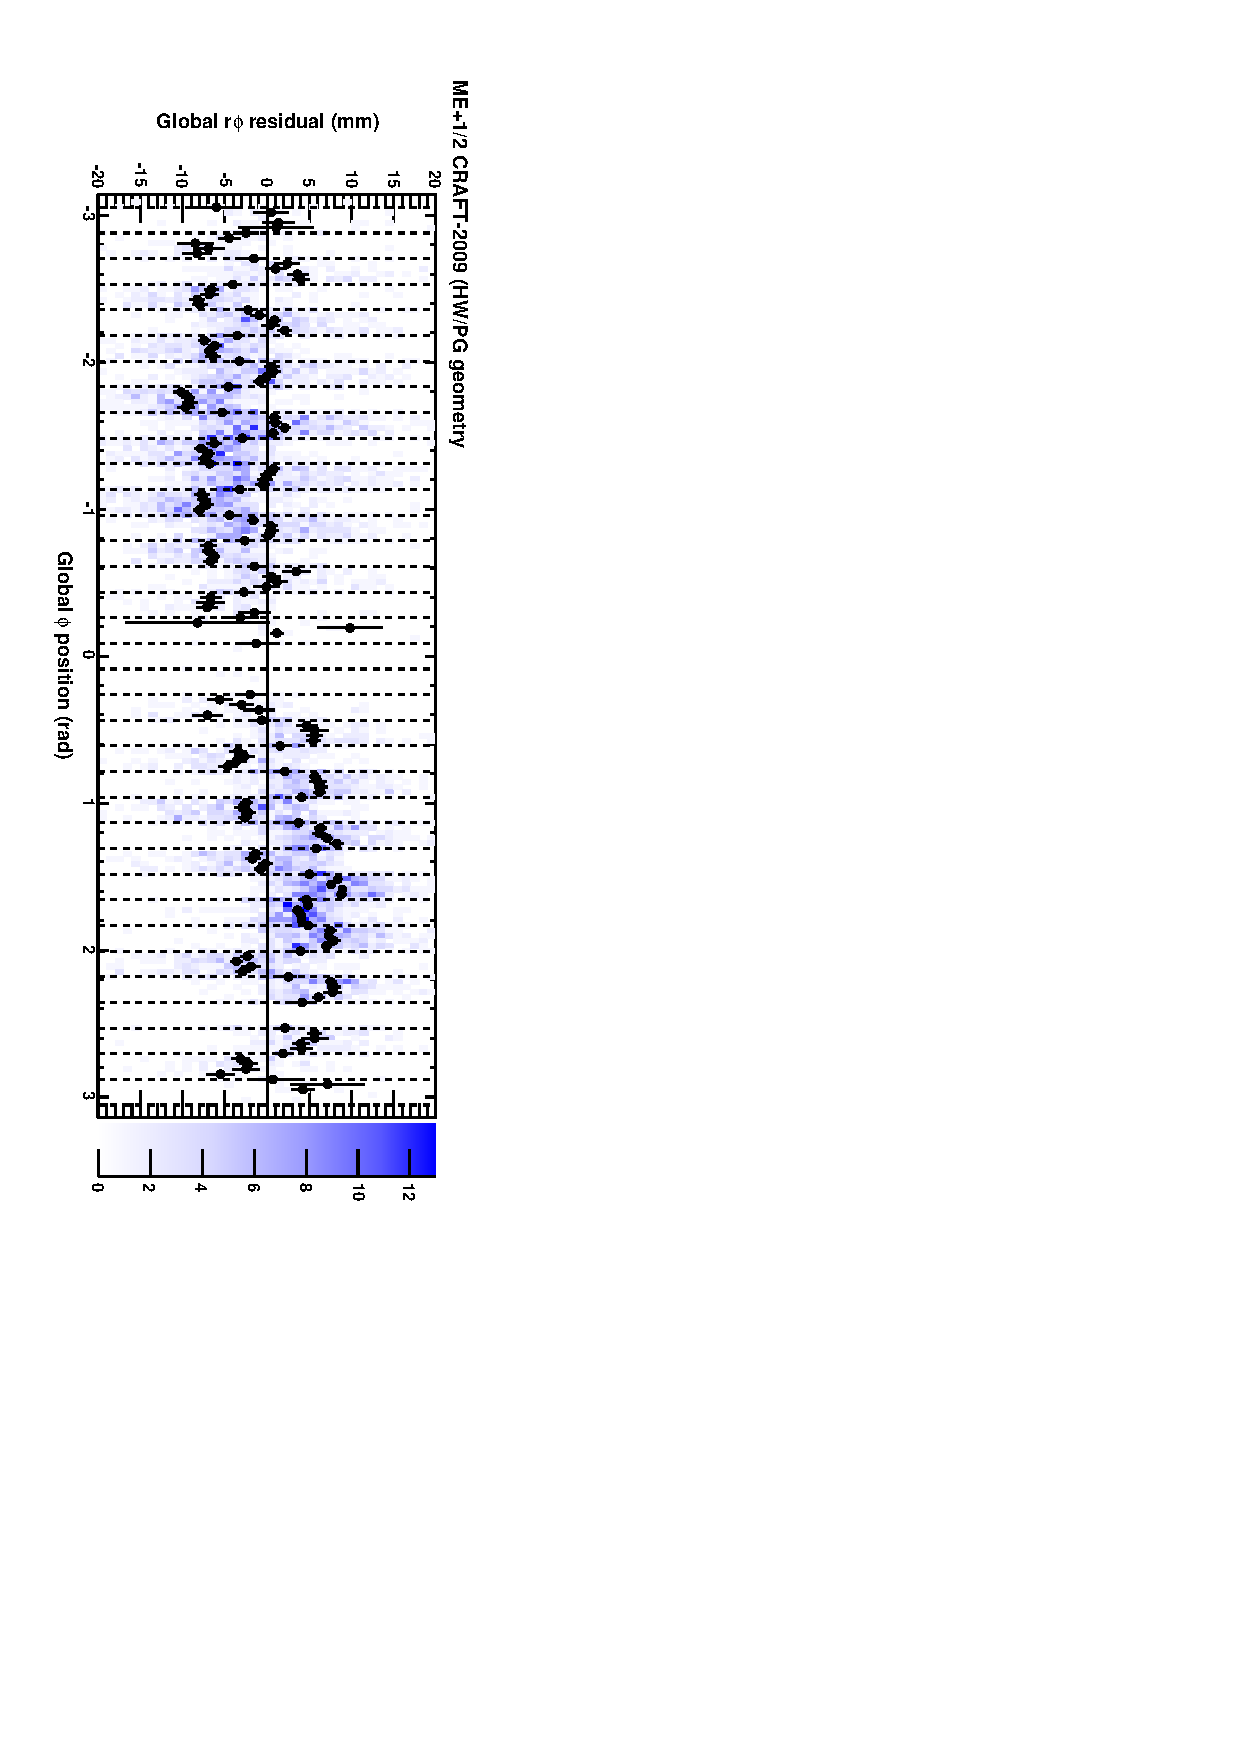
\includegraphics[height=0.75\linewidth, angle=90]{series09.pdf}

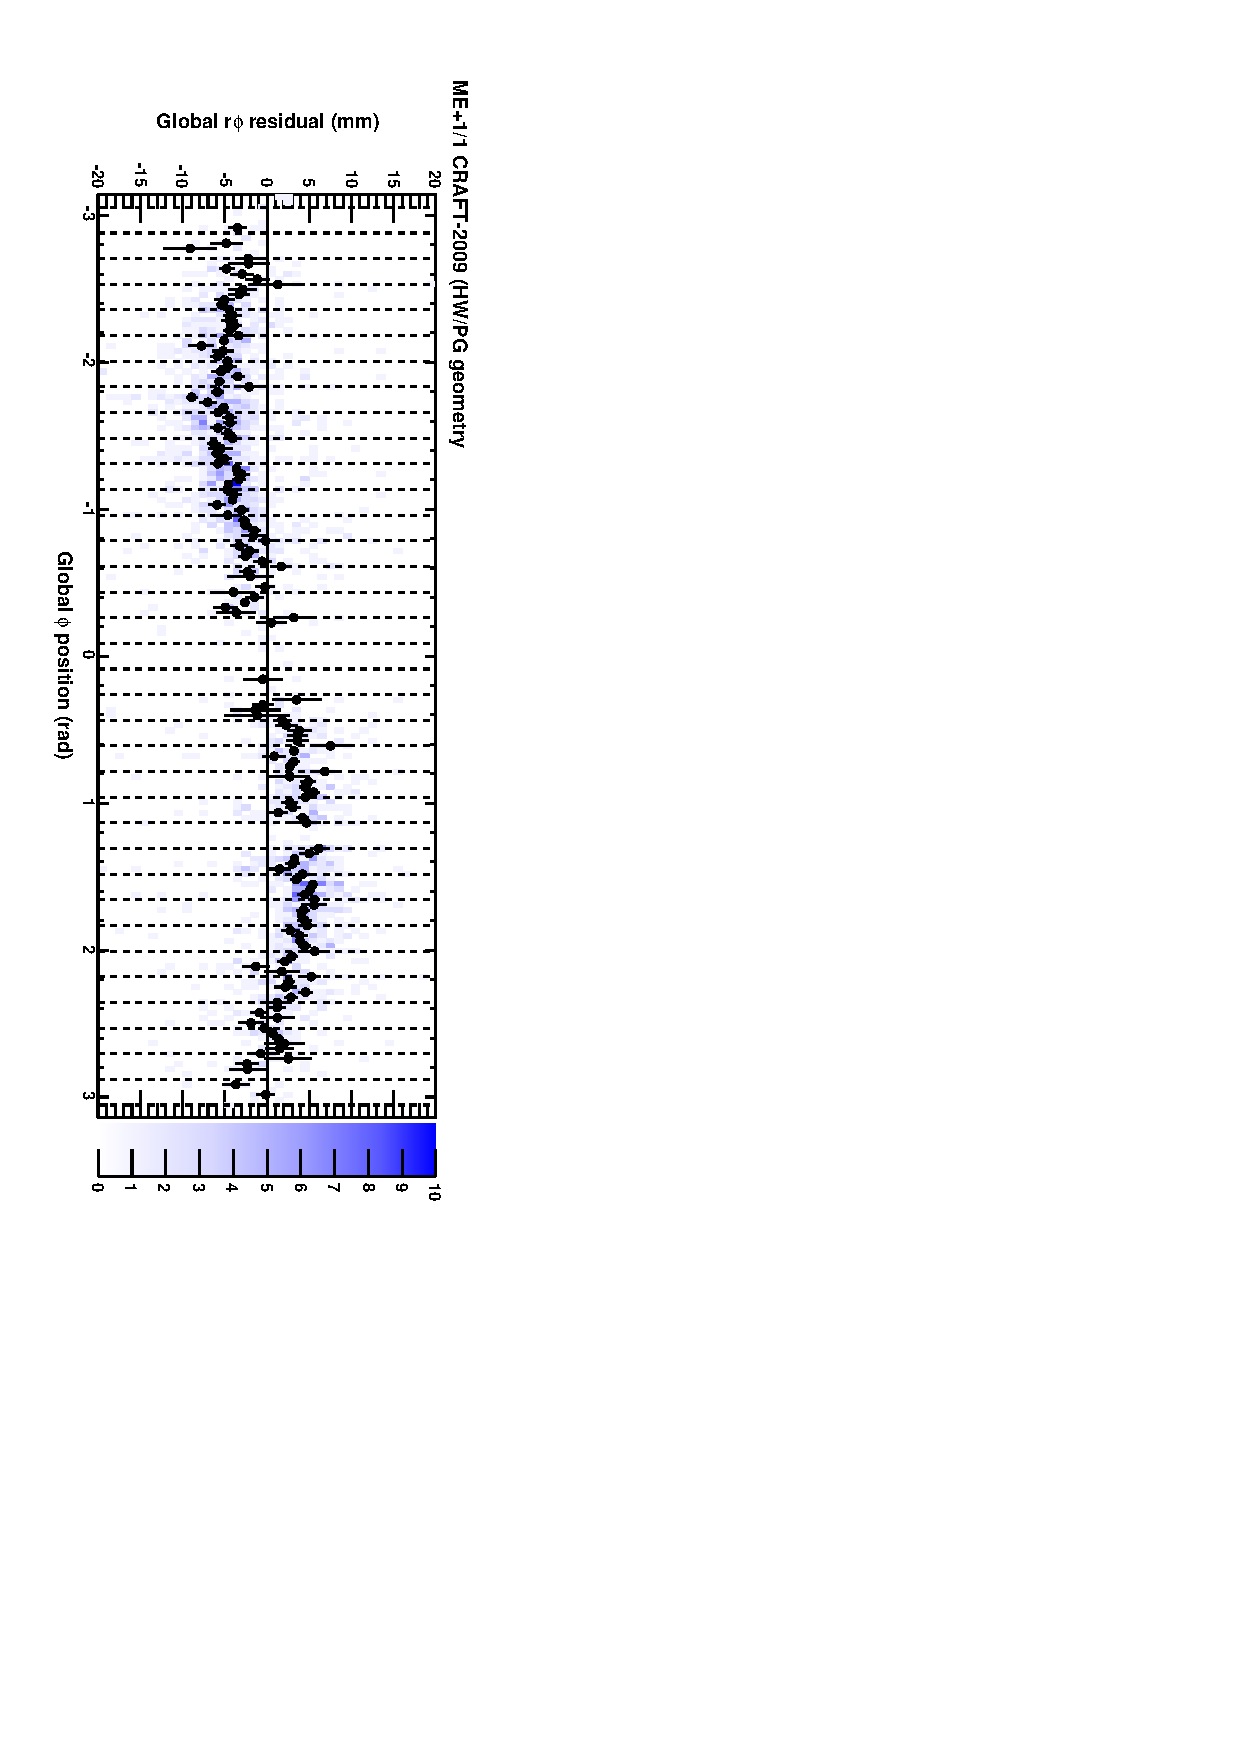
\includegraphics[height=0.75\linewidth, angle=90]{series08.pdf}

\vspace{-2.2 cm}
\hfill clear 5~mm

\hfill $x$ translation

\vspace{2.2 cm}
\vspace{-\baselineskip}
\vspace{-\baselineskip}
\vspace{-\baselineskip}
\vspace{-\baselineskip}
\mbox{ }
\end{frame}

\begin{frame}
\vspace{1 cm}
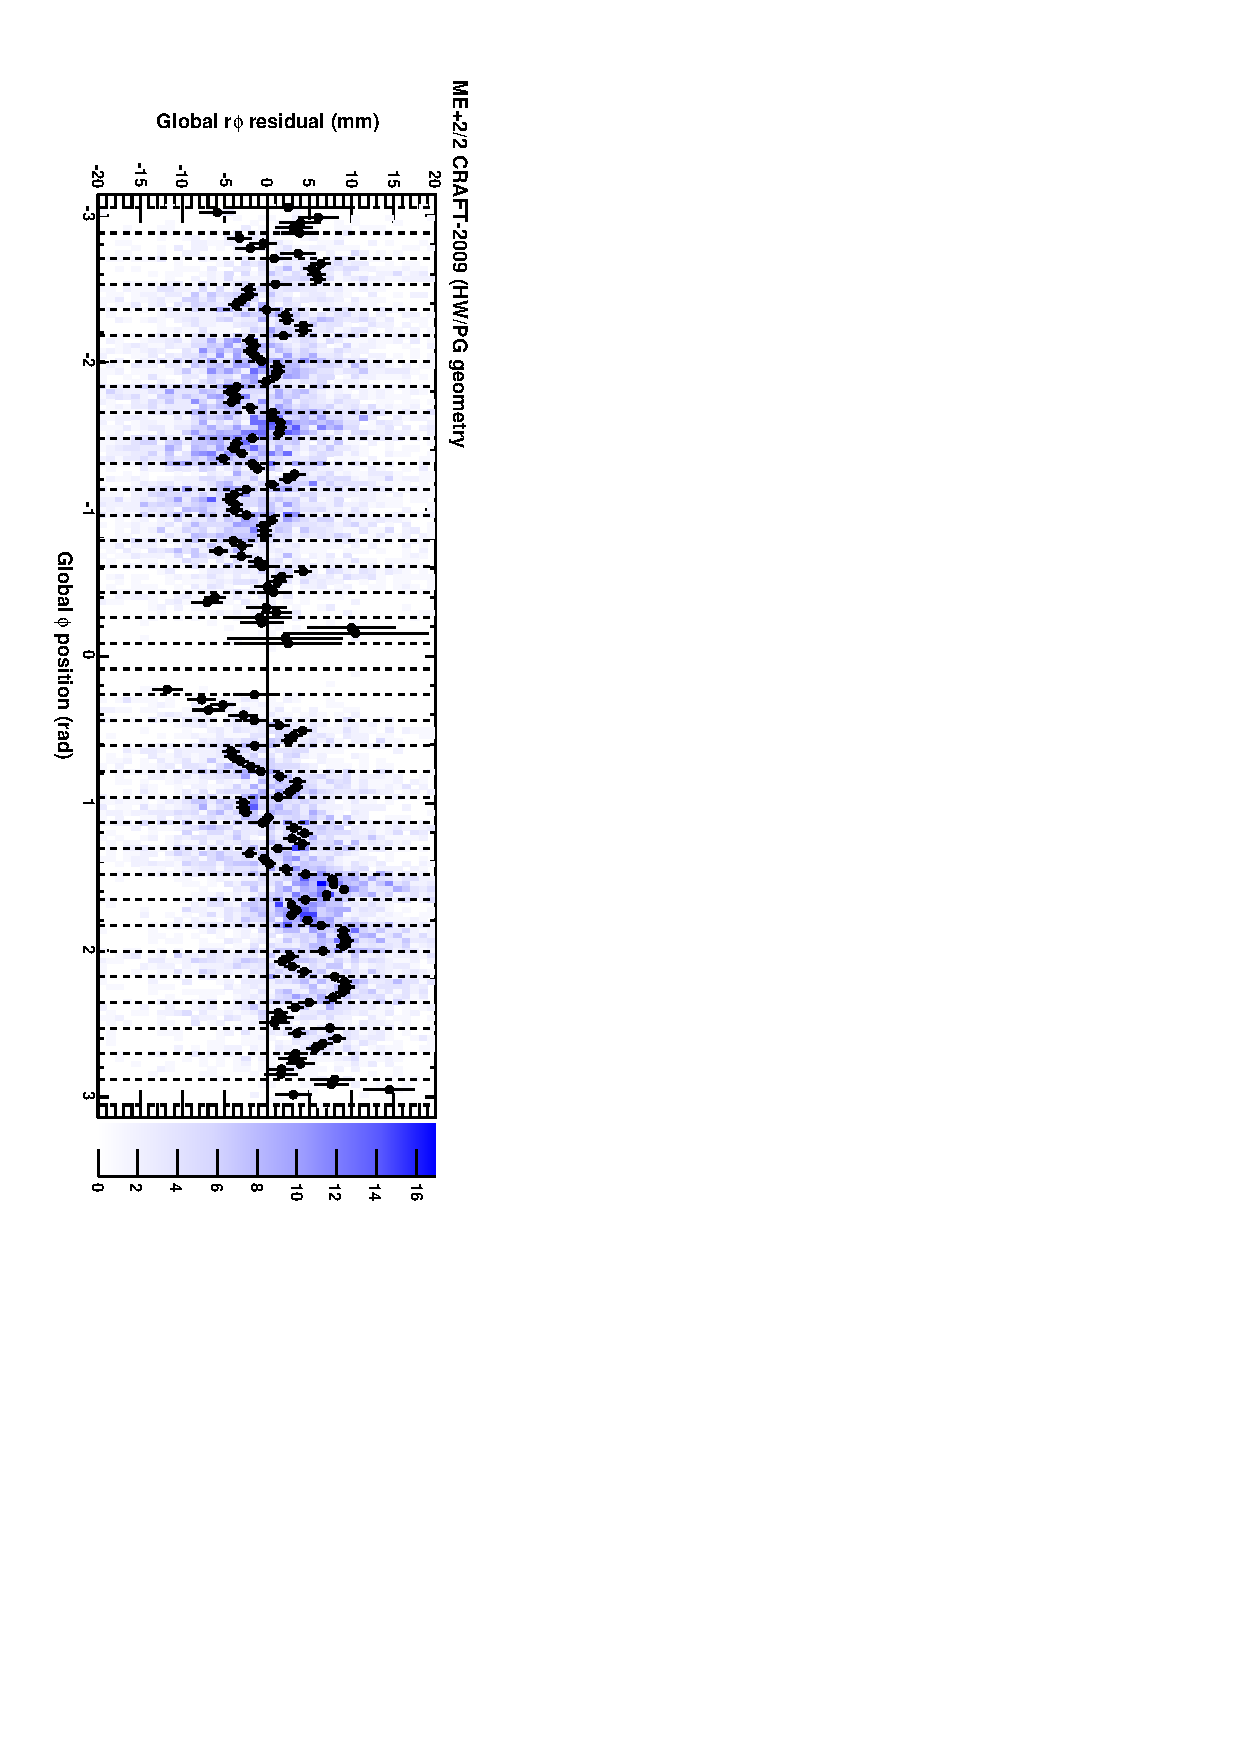
\includegraphics[height=\linewidth, angle=90]{series12.pdf}

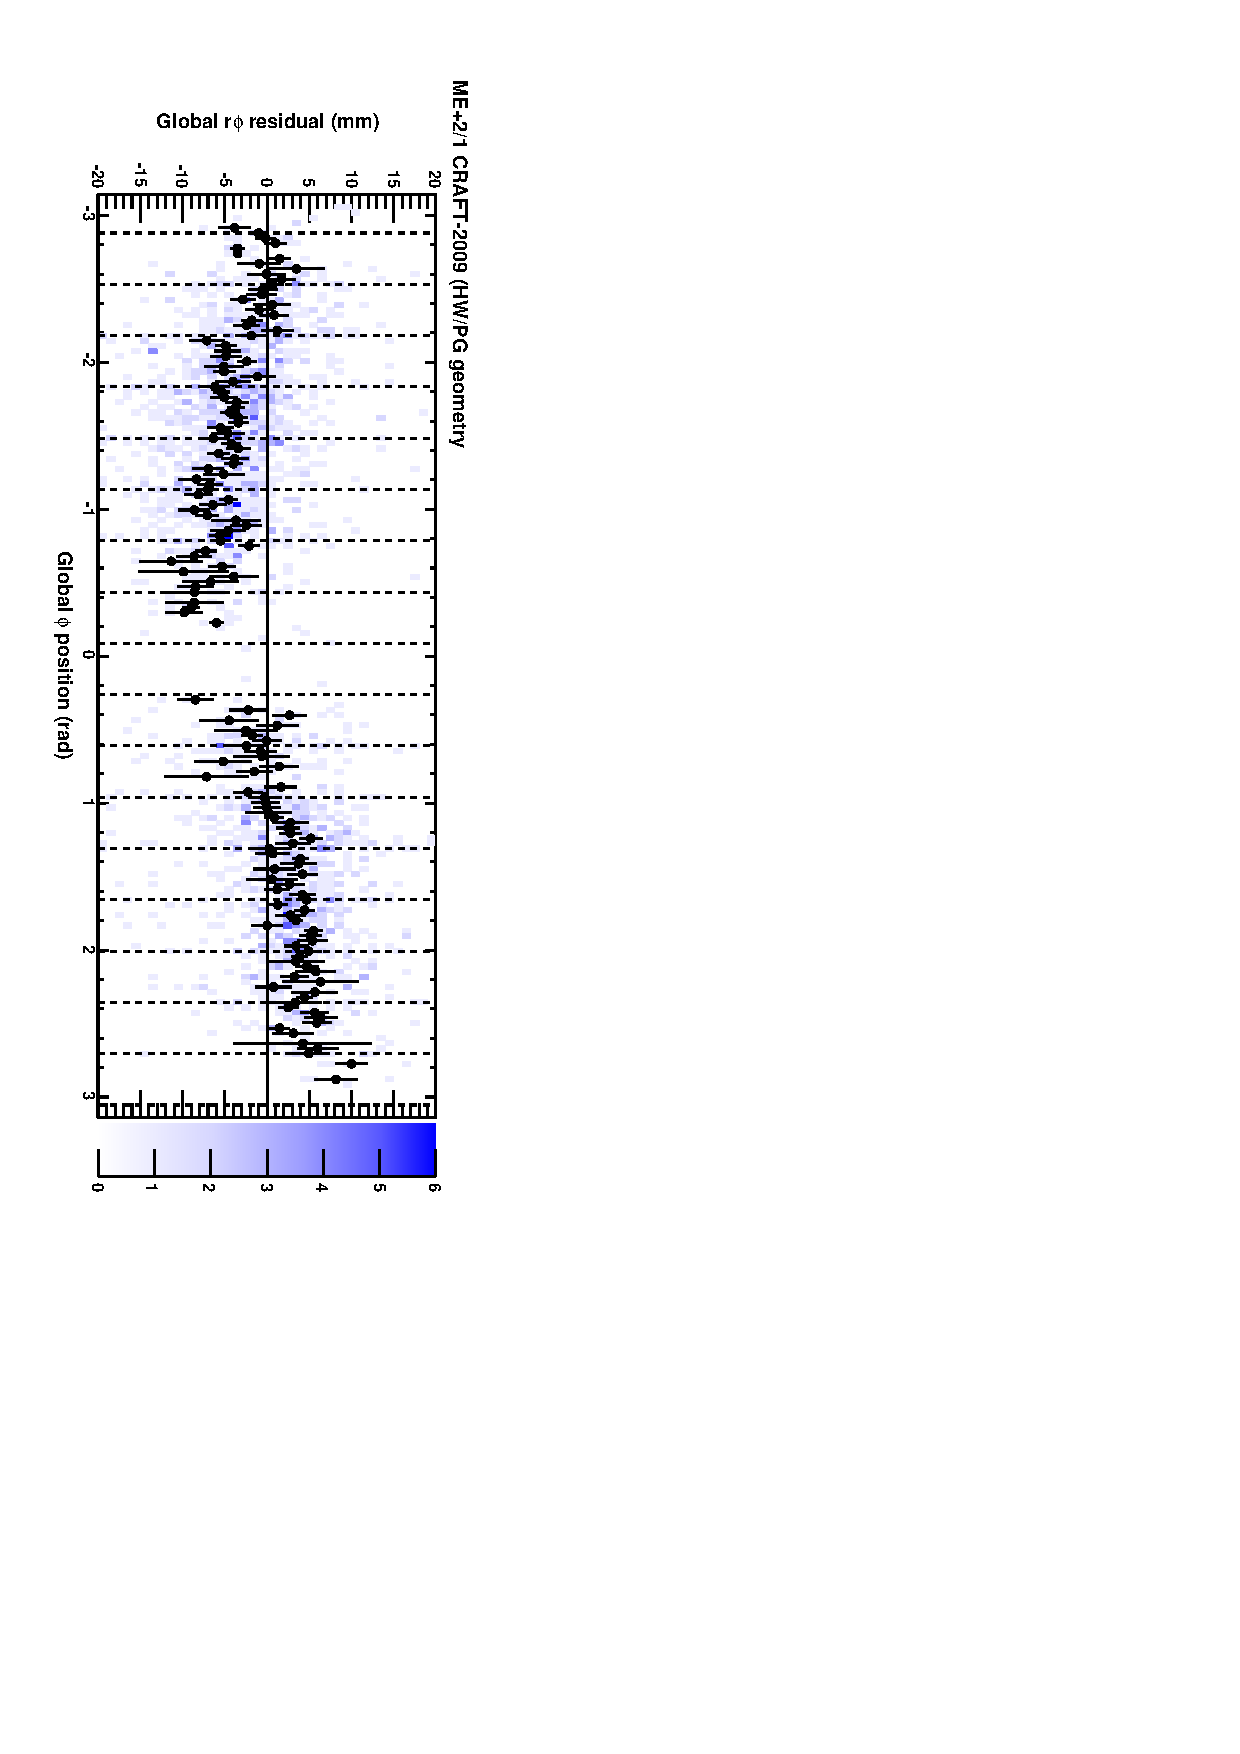
\includegraphics[height=\linewidth, angle=90]{series11.pdf}
\end{frame}

\begin{frame}
\vspace{1 cm}
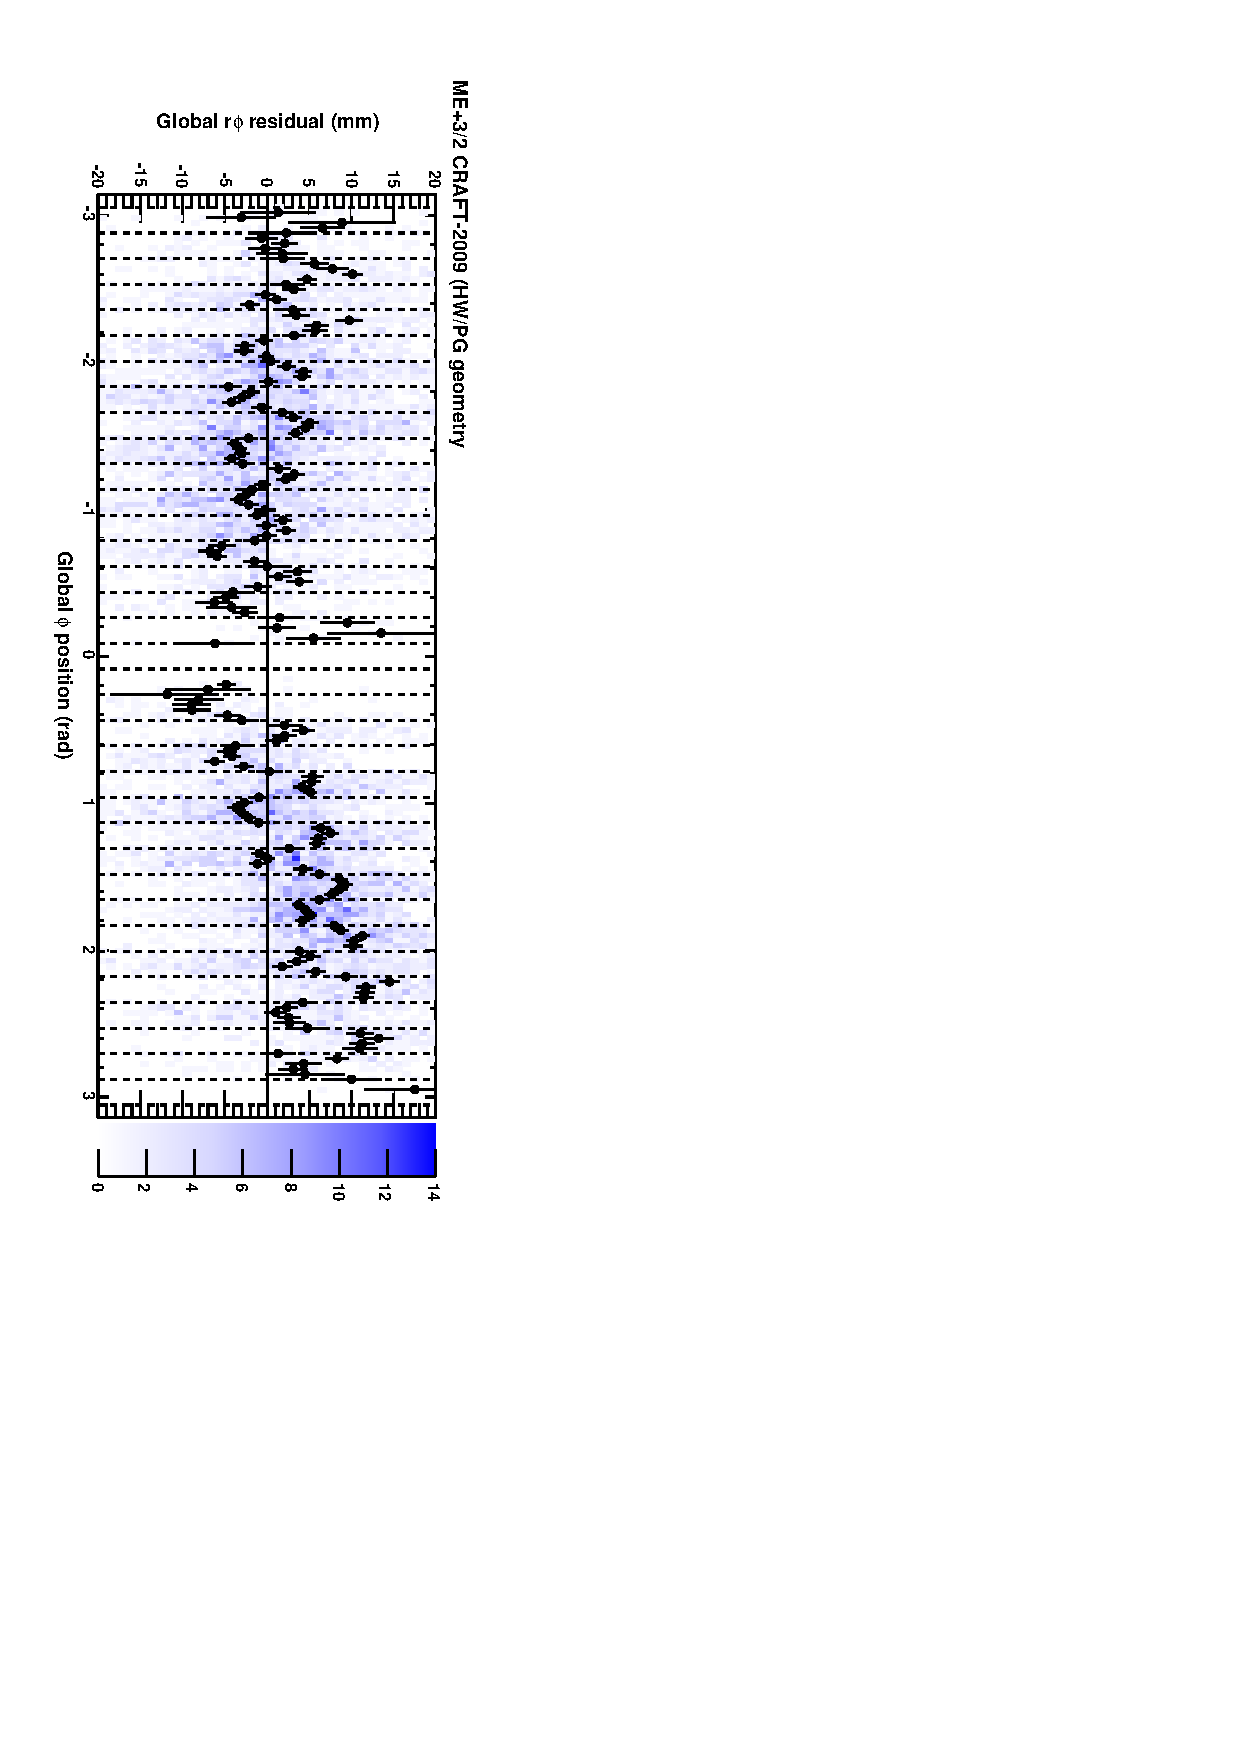
\includegraphics[height=\linewidth, angle=90]{series14.pdf}

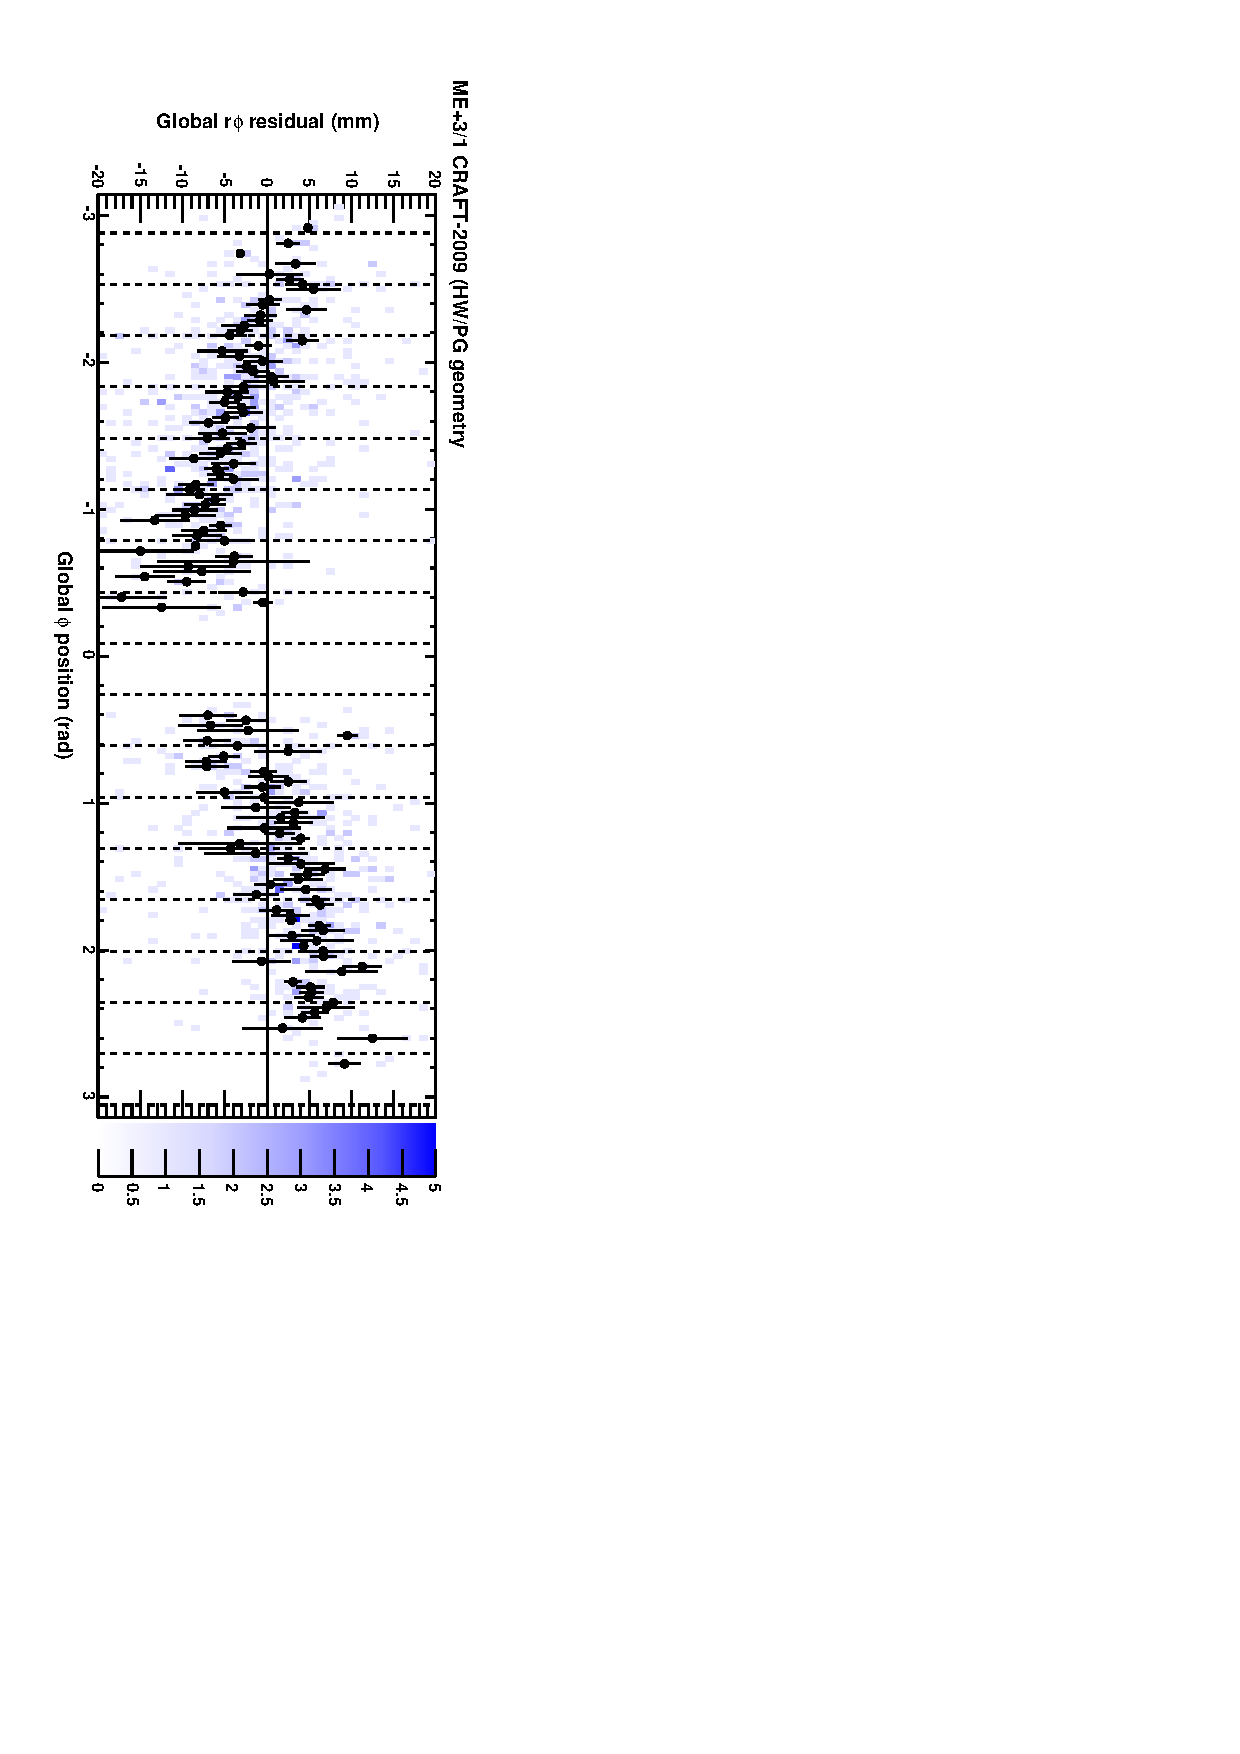
\includegraphics[height=\linewidth, angle=90]{series13.pdf}
\end{frame}

\end{document}
